\documentclass{beamer}
\newtheorem{prop}{Proposition}
\newtheorem{assumption}{Assumption}
\newtheorem{thm}{Thereom}
\newtheorem{corr}{Corollary}

\title[Lanczos and CG]{Lanczos Algorithm and Conjugate Gradient}
\author[Hongda Li, UW]{Hongda Li}
\vspace{-1cm}
\institute[]
{
    {
        \small Applied Mathematics, University of Washington
    }\\
        \vspace{1cm}
    {
        \small {\color{blue}Presented for Something}
    }\\
        \vspace{1cm}
        Still a Draft
}


\date[May ??th 2022]

\AtBeginSection[]
{
  \begin{frame}<beamer>{Outline}
    \tableofcontents[currentsection,currentsubsection]
  \end{frame}
}

\usepackage{biblatex}
\addbibresource{refs.bib}

\begin{document}

\maketitle

\section{Introduction}
    \begin{frame}{Introduction Frame 1}
        \par
        The subjects of discussion are: 
        \begin{itemize}
            \item The Lanczos Algorithm which is used for Tridiagonalizing Sparse Symmetric Matrix $A$, producing the factorizations $Q_k^TAQ_k = T_k$. 
            \item The Conjugate Gradient which is used for solve Positive Definite linear system: $Ax = b$. 
            \item The connections between them and their behaviors under floating point arithematic. 
        \end{itemize}
    \end{frame}


    \begin{frame}{Basics:Krylov Subspace}
        \begin{definition}[Krylov Subspace]
            $$
            \mathcal{K}_k(A|b) = \text{span}( b, Ab, A^2b, \cdots A^{k - 1}b)
            $$
            \begin{itemize}
                \item [1.)] All vectors in the span can be represented in the form of the product matrix polynomial with degree $k - 1$ with vector $b$. 
                \item [2.)] Once the vectors: $b, Ab, A^2b, \cdots A^{k - 1}b$ becomes linearly dependent, the subspace becomes invariant under $A$. 
            \end{itemize}
        \end{definition}
        \begin{definition}[The Grade of Krylov Subspace]
            If the vectors in $\mathcal K_{k}(A|b)$ are linearly dependent and $k$ is the smallest, then the grade of this Krylov Subspace is $k - 1$, denoted as $\text{grade}(A|b)$. 
            \\
            Definition taken from Y. Saad's Textbook: Iterative Methods for Sparse Linear System \cite{book:saad_sparse_linear}
        \end{definition}
    \end{frame}
    
    \begin{frame}{Basics: Projector}
        \begin{definition}[Projectors]
            A matrix $P$ is a projector when $P^2 = P$, we call this property idempotent.    
        \end{definition}
        \begin{itemize}
            \item [1.)] When $P$ is Hermitian, it's an orthogonal projector. 
            \item [2.)] When $P$ is not Hermitian, it's an Oblique projectors
            \item [3.)] The projector $I - P$ projects onto the null space of $P$ and vice versa. 
        \end{itemize}
        
    \end{frame}
    
    \begin{frame}{Basic: Subspace Projection Framework}
        \begin{definition}
            We will choose approximate solutions to our linear system $Ax=b$ from $\mathcal{K}$, and we will orthogonalize the residual $b-A \tilde{x}$ against $\mathcal{L}$.
            \begin{align}
                \text{choose }\tilde{x} \in x_0 + \mathcal{K} \text{ s.t: } b - A\tilde{x} \perp \mathcal{L}.
            \end{align}
            \begin{itemize}
                \item  Characterizes subspace projection methods, such as GMRes, FOM, Bi-CG and CG
            \end{itemize}
        \end{definition}
    \end{frame}
    
    \begin{frame}{Basic: Subspace Projection Framework in Matrix Form}
        \begin{definition}[SPM: Matrix Form]
            Let the columns of $V \in \mathbb{R}^{n \times m}$ be a basis for $\mathcal{K}$ and let the columns of $W \in \mathbb{R}^{n \times m}$ be a basis for $\mathcal{L}$. 
            \begin{align}
                \tilde{x} &= x_0 + Vy
                    \\
                    \text{choose } x \text{ s.t: } b - A\tilde{x}  &\perp \text{ran}(W)
                    \\
                    \implies W^T(b - Ax_0 - AVy) &= \mathbf{0}
                    \\
                    W^Tr_0 - W^TAVy&= \mathbf{0}
                    \\
                    W^TAVy &= W^Tr_0
            \end{align}
        \end{definition}
        
    \end{frame}
    
    \begin{frame}{Basic: Subspace Projection Framework in Matrix Form}
        \begin{definition}[SPM: Matrix Form]
            Let the columns of $V \in \mathbb{R}^{n \times m}$ be a basis for $\mathcal{K}$ and let the columns of $W \in \mathbb{R}^{n \times m}$ be a basis for $\mathcal{L}$. 
            \begin{align}
                \tilde{x} &= x_0 + Vy
                    \\
                    \text{choose } x \text{ s.t: } b - A\tilde{x}  &\perp \text{ran}(W)
                    \\
                    \implies W^T(b - Ax_0 - AVy) &= \mathbf{0}
                    \\
                    W^Tr_0 - W^TAVy&= \mathbf{0}
                    \\
                    W^TAVy &= W^Tr_0
            \end{align}
        \end{definition}
        Observe: 
        \begin{align}
            & \tilde{r} = b - A \tilde{x} = b - A x_0 - AVy = r_0 - AV ( W^T A V )^{-1} W^T r_0
            \\
            & [ A V ( W^T A V )^{-1} W^T ] [ A V ( W^T A V )^{-1} W^T ] = A V ( W^T A V )^{-1} W^T 
        \end{align}
    \end{frame}
    
    \begin{frame}{Basic: Energy Norm Minimizations}
        Alternatively, for some symmetric positive definite matrix $B$, one might choose $\tilde{x} = x_0 + Vy$ to minimize 
            the $B$-norm of the residual $\| r_0 - A V y \|_B = \langle r_0 - A V y , B ( r_0 - A V y ) \rangle^{1/2}$.  Setting the gradient of this function to zero leads to the normal equations:
            \begin{align}
                V^T A^T BAVy = V^T A^T B r_0
            \end{align}
            If $A$ itself is symmetric and positive definite, then we can take $B = A^{-1}$ and minimize the $A^{-1}$-norm of the 
            residual or, equivalently, the $A$-norm of the error $\langle A^{-1} b - \tilde{x} , A ( A^{-1} b - \tilde{x} ) \rangle$.
            The formula for $y$ then becomes
            \begin{align}\label{eqn:Energy_Norm_Minimization_Conditions}
                V^T A V y = V^T r_0
            \end{align}
    \end{frame}
    
    \begin{frame}{Basic: Energy Norm Minimizations}
            Alternatively, for some symmetric positive definite matrix $B$, one might choose $\tilde{x} = x_0 + Vy$ to minimize 
            the $B$-norm of the residual $\| r_0 - A V y \|_B = \langle r_0 - A V y , B ( r_0 - A V y ) \rangle^{1/2}$.  Setting the gradient of this function to zero leads to the normal equations:
            \begin{align}
                V^T A^T BAVy = V^T A^T B r_0
            \end{align}
            If $A$ itself is symmetric and positive definite, then we can take $B = A^{-1}$ and minimize the $A^{-1}$-norm of the 
            residual or, equivalently, the $A$-norm of the error $\langle A^{-1} b - \tilde{x} , A ( A^{-1} b - \tilde{x} ) \rangle$.
            The formula for $y$ then becomes
            \begin{align}\label{eqn:Energy_Norm_Minimization_Conditions}
                V^T A V y = V^T r_0
            \end{align}
            \begin{align}
                & \tilde{r} = r_0 - A V ( V^T A V )^{-1} V^T r_0
                \\
                & [A V (V^T A V )^{-1} V^T ] [ A V ( V^T A V )^{-1} V^T ] = A V ( V^T A V )^{-1} V^T
            \end{align}
    \end{frame}

\section{Driving CG Via CDM}

    \begin{frame}{CG, Lanczos}
        \begin{itemize}
            \item The conjugate direction method can produced applying the subspace projection framework.
            \item The CG method is a special case of the conjugate direction method. 
        \end{itemize}
        Through out the rest of the presentation, we assume: 
        \begin{itemize}
            \item [1)] The matrix $A$ is symmetric positive definite.  
            \item [2)] There is a matrix $P_k = [p_0 \;p_1\;\cdots p_{k-1}]$ whose columns form a basis for the space over which we are minimizing.
        \end{itemize}
    \end{frame}
    
    \begin{frame}{Conjugate Direction Method}
        To solve for $w$, we wish to make $P_k^TAP_k$ to be an easy-to-solve matrix. Let the easy-to-solve matrix be a diagonal matrix and hence we let $P_k$ be a \textit{matrix whose columns are A-Orthogonal vectors}. It's also referred to as \textit{conjugate vectors}. 
        \begin{align}
            P^T_kAP_k &= D_k \text{ where: } (D_k)_{i,i} = \langle p_{i - 1}, Ap_{i - 1}\rangle
            \\
            P_k^T r_0 &= P^T_kAP_kw = D_kw
            \\
            w &= D^{-1}_kP_k^Tr_0
        \end{align}
        Resulting in: 
        \begin{align}
            \begin{cases}
                x_k = x_0 + P_kD^{-1}_kP^T_kr_0
                \\
                r_k = r_0 - AP_kD^{-1}_kP^T_k r_0
            \end{cases}
        \end{align}
    \end{frame}
    \begin{frame}{Conjugate Direction Method}
        Importantly, $P_kD_k^{-1}P_k^Tr_0, AP_kD_k^{-1}P_k^Tr_0$ are oblique pojectors.
        \\
        For convenience, we denote $\overline{P}_k = P_kD_k^{-1}P_k^{T}$; So we can simply denotes them by $A\overline{P}_k, \overline{P}_kA$. Observe that: 
        \begin{align}
            & \text{ran}(I - A\overline{P}_k )\perp \text{ran}(P_k)
            \\
            & \text{ran}(I - \overline{P}_kA) \perp \text{ran}(AP_k)
        \end{align}
    \end{frame}
    \begin{frame}{Generating Orthogonal Vector}
        \begin{prop}[Generating $A$-Orthogonal Vectors]
            Given any set of linearly independent vectors, for example $\{u_i\}_{i = 0}^{n - 1}$, one can generate a set of A-Orthogonal vectors from it. More specifically:
            \begin{align}
                p_k &= (I - \overline{P}_kA)u_k \implies p_k \perp \text{ran}(AP_k)
            \end{align}
        \end{prop}
        
    \end{frame}
    \begin{frame}{Conjugate Direction Method}
        The method is acually mentioned by Hestenes, Steifel back in 1952\cite{paper:cg_original}. 
        \begin{definition}[Conjugate Direction Method]
            \begin{align}\small
                \begin{cases}
                    \overline{P}_k = P_kD^{-1}_kP_k^T
                    \\
                    x_k = x_0 + \overline{P}_k r_0
                    \\
                    r_k = (I - A\overline{P}_k) r_0
                    \\
                    P^T_kAP_k = D_k
                    \\
                    p_k = (I - \overline{P}_kA)u_k & \{u_i\}_{i = 0}^{n - 1} \text{ linearly independent vectors}
                \end{cases}
            \end{align}
        \end{definition}
        \begin{itemize}\small
            \item With the assistance of a set of basis vectors that span the whole space, this algorithm can achieve the objective Improvement can be made 
            \item Would be great if we could update $x_k$, $r_k$, and $p_k$ using results from previous iterations.
            \item When $\{u_i\}_0^{n - 1}$ is the set of standard basis vector, the method is equivalent to the Gauss Eliminations
        \end{itemize}
    \end{frame}
    \begin{frame}{CDM Update: }
        I did some math and here is the update: 
        \begin{align}
            r_k - r_{k - 1} &= r_0 - A\overline{P}_kr_0 - (r_0 - A\overline{P}_{k - 1}r_0)
            \\
            x_{k} - x_{k - 1} &= 
                    p_{k - 1}\frac{\langle p_{k - 1}, r_0\rangle}{\langle p_{k - 1}, Ap_{k - 1}\rangle}
            \\
            a_{k - 1} &:= \frac{\langle p_{k - 1}, r_0\rangle}{
                        \langle p_{k - 1}, Ap_{k - 1}\rangle
                    } = 
                    \frac{\langle p_{k - 1}, r_{k - 1}\rangle}{
                        \langle p_{k - 1}, Ap_{k - 1}\rangle
                    }
            \\
            p_k &= (I - \overline{P}_kA)u_k
        \end{align}
    \end{frame}
    \begin{frame}{Conjugate Gradient}
        By setting $\{u_i\}_{i = 0}^{n - 1}$ we derive the conjugate gradient algorithm. To get the magic, we introduce these lemmas: 
        \begin{lemma}[CG Lemma 1]\small
            \begin{align}
                    \langle p_{j}, Ap_k\rangle
                    &=\langle r_k, Ap_{j}\rangle
                    = \langle p_{j}, Ar_k\rangle \quad 0 \le j \le k 
            \end{align}
        \end{lemma}
        \begin{lemma}[CG Lemma 2]\small
            \begin{align}
                \langle r_k, p_k\rangle &= \langle r_k, r_k\rangle
            \end{align}
        \end{lemma}
        
    \end{frame}
    \begin{frame}{Conjugate Gradient}
        \begin{prop}[CG Generates Orthogonal Residuals]\small
            \begin{align}
                \langle r_k , r_j \rangle = 0 \quad \forall\; 0 \le j \le k - 1 
            \end{align}
        \end{prop}
        We skip the proof for the presentation. 
    \end{frame}
    \begin{frame}{CG: Recurrence}
        \begin{prop}[CG Recurrences]
            \begin{align}
                p_k &= r_k + b_{k - 1}p_{k - 1} \quad b_{k - 1} = \frac{\Vert r_k\Vert_2^2}
                {\Vert r_{k - 1}\Vert_2^2}
            \end{align}
        \end{prop}
    \end{frame}
    \begin{frame}{CG: Recurrence Proof}
        \begin{align}
            p_k &= (I - \overline{P}_kA)r_k 
            \\
            &= r_k - \overline{P}_kAr_k = 
            r_k - P_kD^{-1}_kP^T_kAr_k
            \\
            &= r_k - P_kD^{-1}_k(AP_k)^Tr_k
            \\
            (AP_k)^Tr_k &= 
            \begin{bmatrix}
                \langle p_0, Ar_k\rangle
                \\
                \langle p_1, Ar_k\rangle
                \\
                \vdots
                \\
                \langle p_{k - 1}, Ar_k\rangle
            \end{bmatrix}
        \end{align}
        
    \end{frame}
    \begin{frame}{CG Recurrence Proof}
        \begin{align}
            \langle p_j, Ar_k\rangle& \quad \forall\; 0 \le j \le k -2 
            \\
            \langle p_j, Ar_k\rangle&= \langle r_k, Ap_j\rangle
            \\
            &= \langle r_k, a_j^{-1}(r_j - r_{j + 1})\rangle
            \\
            &= a_j^{-1}\langle r_k, (r_j - r_{j + 1})\rangle = 0
        \end{align}
        \begin{itemize}
            \item[(41)] By the second lemma. 
            \item[(42)] By the CDM Recurrences
            \item[(43)] By the orthogonality of the residual vectors 
        \end{itemize}
    \end{frame}
    \begin{frame}{CG Recurrence Proof}
        \begin{align}
            (AP_k)^Tr_k &= 
            \begin{bmatrix}
                \langle p_0, Ar_k\rangle
                \\
                \langle p_1, Ar_k\rangle
                \\
                \vdots
                \\
                \langle p_{k - 1}, Ar_k\rangle
            \end{bmatrix}
            = 
            a_{k - 1}^{-1}\langle r_k, (r_{k - 1} - r_{k})\rangle \xi_k
        \end{align}
        $\xi_k$ is the $k$th standard basis vector in $\mathbb R^k$. We are almost there. 
    \end{frame}
    \begin{frame}{CG Recurrence Proof}
        \begin{align}
            p_k &= r_k - P_kD^{-1}_k(AP_k)^Tr_k
            \\
            &= r_k - P_kD_k^{-1}a_{k - 1}^{-1}(\langle r_k, (r_{k - 1} - r_{k})\rangle) \xi_k
            \\
            &= 
            r_k - \frac{a_{k -1}^{-1}\langle -r_k, r_k\rangle}
            {\langle p_{k - 1}, Ap_{k - 1}\rangle}p_k
            \\
            &= r_k + \frac{a_{k -1}^{-1}\langle r_k, r_k\rangle}
            {\langle p_{k - 1}, Ap_{k - 1}\rangle}p_k
            \\
            &= r_k + 
            \left(
                \frac{\langle r_{k - 1}, r_{k - 1}\rangle}{\langle p_{k - 1}, Ap_{k - 1}\rangle}
            \right)^{-1}
            \frac{\langle r_k, r_k\rangle}{\langle p_{k - 1}, Ap_{k - 1}\rangle}p_k
            \\
            &= 
            r_k + \frac{\langle r_k, r_k\rangle}{\langle r_{k - 1}, r_{k - 1}\rangle}p_k
        \end{align}
        Done. This is presented because it will be useful for partially orthgonalized CG later. 
    \end{frame}
    \begin{frame}{The CG Algorithm}
        \begin{definition}[CG]\label{def:CG}
                \begin{align}
                    & p^{(0)} = b - Ax^{(0)} 
                    \\&
                    \text{For } i = 0,1, \cdots
                    \\&\hspace{1.1em}
                    \begin{aligned}
                        & a_{i} = \frac{\Vert r^{(i)}\Vert^2}{\Vert p^{(i)}\Vert^2_A}
                        \\
                        & x^{(i + 1)} = x^{(i)} + a_i p^{(i)}
                        \\
                        & r^{(i + 1)} = r^{(i)} - a_iAp^{(i)}
                        \\
                        & b_{i} = \frac{\Vert r^{(i + 1)}\Vert_2^2}{\Vert r^{(i)}\Vert_2^2}
                        \\
                        & p^{(i + 1)} = r^{(i + 1)} + b_{i}p^{(i)}
                    \end{aligned}
                \end{align}
            \end{definition}
    \end{frame}
    \begin{frame}{CG and Krylov Subspace}
        \begin{theorem}[CG and Krylov Subspace]\label{theorem:CG_and_Krylov_Subspace}
                    \begin{align}
                        \text{choose: } x_k\in x_0 + \mathcal K_{k}(A|r_0) \text{ s.t: } r_k \perp \mathcal K_{k}(A|r_0)
                    \end{align}    
        \end{theorem}
        Take note that, $\text{ran}(P_k) = \mathcal K_k(A|r_0)$ because the index starts with zero for the gonjugate vectors.
        \begin{itemize}
            \item The number of iterations before termination is just the grade of Krylov Subspace. 
            \item Something that is special unique compare to CDM. 
            \item Provides connections to the Lanczos Algorithm.
        \end{itemize}
    \end{frame}
\section{Lanczos iterations as a Symmetric case of Arnoldi iterations}
    \begin{frame}{The Arnoldi Iteration}
        This is a matrix of upper Hessenberg form: 
        \begin{align}
            \tilde{H}_k = 
            \begin{bmatrix}
                h_{1, 1} & h_{1, 2} & \cdots & h_{1, k} 
                \\
                h_{1, 2} & h_{2, 2} & \cdots & h_{2, k}
                \\
                \\
                & \ddots & &\vdots
                \\
                & & h_{k, k - 1}& h_{k, k}
                \\
                & & & h_{k + 1, k}
            \end{bmatrix}
        \end{align}
        \begin{align}
                Q_1 &= q_1
                \\
                (\tilde{H}_k)_{j + 1, k}q_{j + 1}&= (I - Q_jQ_j^H)Aq_j
                \\
                (\tilde{H}_j)_{1:j, j} &= Q_jQ_j^HAq_j
        \end{align}
        Usually when implementing, the subdiagonal of $H_k$ are chosen to be 
        \begin{align}
            \tilde H_{k + 1, k} := \Vert (I - Q_kQ_k^T)Aq_k\Vert
        \end{align}
    \end{frame}
    \begin{frame}{Arnoldi Recurrence}
        \begin{align}
                AQ_{k} &= Q_{k + 1}\tilde{H}_k
                \\
                Q_{k}^HAQ_{k} &=: H_k
        \end{align}
        We define $H_k$ to be the principal submatrix of $\tilde{H}_k$. Please observe that, if $A$ is symmetric, then $Q^H_kAQ_k$ is also symmetric, which makes $H_k$ symmetric, implying $H_k$ is a symmetric tridiagonal Matrix, giving us the tridiagonal factorization of $A$. 
        \begin{itemize}
            \item The characteristic polynomial of $H$, minimizes $\Vert p(A|w)q_1\Vert_2$ among all monic polynomials\cite{book:trefethen}.
            \item $\text{ran}(Q_k) = \mathcal K_k(A|q_1)$. Range of $Q_k$ spans $\mathcal K_k(A|q_1)$.
            \item Terminates when $k = \text{grade}(A|q_1)$. 
        \end{itemize}
    \end{frame}
    \begin{frame}{Lanczos Recurrences}
        \begin{theorem}[Lanczos Recurrences]
            $T_k$ is a symmetric tridiagonal matrix with $a_i, 1\le i\le k$ on the diagonal and $\beta_i, 1 \le i \le k -1$ on the sub/super diagonal. 
            \begin{align}
                AQ_k &= Q_kT_k + \beta_k q_{k + 1}\xi_k^T = Q_{k + 1}\tilde{T}_k
                \\
                \implies Aq_j
                &= \beta_{j - 1}q_{j - 1} + \alpha_j q_j + \beta_{j}q_{j + 1} \quad \forall\; 2\le j\le k
                \\
                \implies Aq_1 &= \alpha_1q_1 + \beta_1 q_2
            \end{align}    
        \end{theorem}
    \end{frame}
    \begin{frame}{Minimal Monic of Lanczos}
        We use the property minimal monic property of Arnoldi, and the eigen decomposition for $A$. 
         \begin{align}
                & \min_{p_{k - 1}:\text{monic}} \Vert p(A)q_1\Vert_2
                \\
                & =\Vert \overline{p}_{k - 1}(A)q_1\Vert_2
                \\
                & = \Vert V \bar{p}_{k - 1}(\Lambda)V^Tq_1\Vert_2
                \\
                & = \Vert \bar{p}_{k - 1}(\Lambda)V^Tq_1\Vert_2
                \\
                &= \sqrt{
                    \sum_{i = 1}^n p_{k - 1}(\lambda_i)^2(V^Tq_1)^2_1
                }
            \end{align}
            The last line is saying the characteristic polynomial for $T_k$ from the Lanczos iterations is minimizing a weighted squared sum at the eigenvalues of the matrix $A$. 
    \end{frame}
    \begin{frame}{Extra Useful Facts}
        \begin{itemize}
            \item [1.)] $q_k$ generated by Lanczos, which is a polynomial under $\mathcal K_k(A|q_1)$, is orthogonal under the weighted discrete measure defined by a weighted inner product at eigenvalues of $A$. 
            \item [2.)] The characteristic polynomial of $T_k$ is a scaled version of the polynomial for $q_k$, which means they are also orthogonal. 
            \item [3.)] Lanczos produces a symmetric tridiagonal matrix with non zero on the sub/super diagonal, that matrix has no repeated eigenvalues. 
        \end{itemize}
    \end{frame}
\section{CG Exact Convergence}
    \begin{frame}{CG Exact Convergence Rate}
        {\footnotesize
        \begin{align}
            \Vert e_k\Vert_A^2 & =
            \min_{x_k \in x_0 + \mathcal K_k(A|r_0)}
            \Vert 
                x^+ - x_k
            \Vert_A^2
            \\
            x_k \in x_0 + \mathcal K_k(A|r_0) 
            & \implies
            e_k = e_0 + p_{k - 1}(A|w)r_0
            \\
            \implies  &=
            \min_{w\in \mathbb R^k}
            \Vert 
                e_0 + p_{k - 1}(A|w)r_0
            \Vert_A^2
            \\
            &= \min_{w\in \mathbb R^k}
            \Vert 
                e_0 + Ap_{k - 1}(A|w)e_0
            \Vert_A^2
            \\
            &= \min_{w\in \mathbb R^k}
            \Vert 
                A^{1/2}(I + Ap_{k - 1}(A|w))e_0
            \Vert_2^2
            \\
            &\le
            \min_{w\in \mathbb R^k}
            \Vert 
                I + Ap_{k - 1}(A|w)
            \Vert_2^2\Vert e_0\Vert_A^2 \quad 
            \\
            & = 
            \min_{w\in \mathbb R^k}
            \left(
                \max_{i = 1, \dots, n}
                |1 + \lambda_i p_{k - 1}(\lambda_i|w)|^2
            \right)\Vert e_0\Vert_A^2
            \quad
            \\
            & \le 
            \min_{w\in \mathbb R^k}
            \left(
                \max_{x\in [\lambda_{\min}, \lambda_{\max}]}
                |1 + \lambda_i p_{k - 1}(\lambda_i|w)|^2
            \right)\Vert e_0\Vert_A^2
            \quad 
            \\
            &= 
            \min_{p_{k}: p_{k}(0) = 1}
            \max_{x\in [\lambda_{\min}, \lambda_{\max}]}
            | p_{k}(x)|^2 \Vert e\Vert_A^2
            \\
            \implies
            \frac{\Vert e_k\Vert_A}{\Vert e_0\Vert_A} &\le 
            \min_{p_{k}: p_{k}(0) = 1}\max_{x\in [\lambda_{\text{min}}, \lambda_{\text{max}}]} |p_{k}(x)|   
        \end{align}
        }
    \end{frame}
    \begin{frame}{CG Exact Convergence Rate}
        \begin{itemize}
            \item It's minimizing the using a polynomial $p_k(x)$ that has $p(0) = 1$. 
            \item To bound it, one can use the inf norm minimization property of Chebyshev Polynomial.
            \item Similar to what was taught in AMATH 585 2022 Winter. 
        \end{itemize}
        Using chebyshev polynomial, one can derive the bound: 
        \begin{align}
            \frac{\Vert e_k\Vert_A}{\Vert e_k\Vert_A}
            \le 2 \left(
                    \frac{\sqrt{\kappa} + 1}{\sqrt{\kappa} - 1}
            \right)^k
        \end{align}
        \begin{itemize}
            \item Bound can be improved if we assume single outlier eigenvalues, or a cluster of outlier eigenvalues away from the origin. 
        \end{itemize}
    \end{frame}
    \begin{frame}{Lanczos Conjugate Equivalence}
        We had been brewing the fact that the Iterative Lanczos Algorithm and the Conjugate gradient algorithm are related. From the previous discussion we can observe that: 
        \begin{enumerate}
            \item [1.)] Both Lanczos and CG terminates when the grade of Krylov subspace is reached. For Lanczos it's $\mathcal K_k(A|q_1)$ and for CG it's $\mathcal K_k(A|r_0)$.
            \item [2.)] Both Lanczos and CG generate orthogonal vectors, for Lanczos they are the $q_i$ vector and for CG they are the $r_i$ vectors. 
        \end{enumerate}
    \end{frame}
    \begin{frame}{Lanczos Vectors and Residuals of CG}
        Lanczos Vectors are residuals of CG, but unit length and pointing at opposite directions at every other iterations. 
        \begin{align}
                q_1 &= \hat r_0\\
                q_2 &= -\hat r_1
                \\
                \vdots
                \\
                q_j &= (-1)^{j + 1}\hat r_{j + 1}
        \end{align}
    \end{frame}
    \begin{frame}{Generatin Tridiagonal Matrix of Lanczos from CG Parameters}
        The tridiagonal matrix of the equivalent Lanczos can be obtained from the CG parameters. 
        \begin{align}
            \begin{cases}
                \alpha_{j + 1} = \frac{1}{a_j} + \frac{b_{j - 1}}{a_{j - 1}}
                & \forall 1 \le j \le k - 1
                \\
                \beta_{j} = \frac{\sqrt{b_{j - 1}}}{a_{j - 1}}
                & \forall 2 \le j \le k - 2 
                \\
                \alpha_1 = a_0^{-1} & 
                \\
                \beta_1 = \frac{\sqrt{b_0}}{\alpha_0}
            \end{cases}
        \end{align}
        \begin{itemize}
            \item Still works fine even if $A$ is indefinite, if we have the luck of $a_j$ being non zero. 
        \end{itemize}
    \end{frame}
    \begin{frame}{From Lanczos to CG}
         CG is a special case of applying the Lanczos Iterations with $q_1 = r_0$ to a positive definite matrix. However there are still questions left. 
        \begin{enumerate}
            \item [1.)] How are the solutions $x_k$ generated by CG related to the Lanczos Iterations? 
            \item [2.)] How are the A-Orthogonal vectors $p_k$ from CG related to Lanczos?
        \end{enumerate}
        To answer it we need to derive CG using the Lanczos iterations. 
    \end{frame}
    \begin{frame}{From Lanczos to CG}
         we initialize $q_1 = \hat{r}_0$, then the following relationship between Lanczos and CG occurs between their parameters: 
        \begin{align}
            \begin{cases}
                y_k = T^{-1}_k \beta\xi_1
                \\
                x_k = x_0 + Q_k y_k
                \\
                r_k = -\beta_{k}\xi_k^T y_k q_{k +1}
            \end{cases}
        \end{align}
    \end{frame}
    \begin{frame}{From Lanczos to CG}
        To start recall that the Lanczos Algorithm Asserts the following recurrences:
        \begin{align}
            AQ_k = Q_{k + 1} \begin{bmatrix}
                T_k
                \\
                \beta_k \xi_k^T
            \end{bmatrix}
        \end{align}
        we know that: $p_k \in \mathcal K_{k + 1}(A|r_0)$, the matrix $P_k, Q_k$ spans the same subspace, and that means: 
        \begin{align}
            x_{k + 1} &= x_0 + Q_ky_k
            \\
            r_{k + 1} &= r_0 - AQ_k y_k
            \\
            Q^H_kr_{k + 1} &= Q_k^H r_0 - Q_k^HAQ_k y_k
            \\
            \implies
            0 &= \beta\xi_1 - T_k y_k
            \\
            y_k &= T_k^{-1}\beta \xi_1
        \end{align}
    \end{frame}
    \begin{frame}{From Lanczos to CG}
        \begin{align}
            r_{k + 1} &= r_0 - AQ_k y_k
            \\
            &= r_0 - AQ_k T_k^{-1}\beta \xi_1
            \\
            \implies
            &= \beta q_1 - AQ_k T_k^{-1} \beta\xi_1
            \\
            &= \beta q_1 - Q_{k + 1}\begin{bmatrix}
                T_k \\ \beta_k \xi_k^T
            \end{bmatrix}T_k^{-1} \beta\xi_1
            \\
            &= \beta q_1 - 
            (Q_k T_k + \beta_k q_{k + 1}\xi_k^T)T_k^{-1} \beta\xi_1
            \\
            &= 
            \beta q_1 - (Q_k \beta \xi_1 + \beta_k q_{k + 1}\xi_{k + 1}T_k^{-1}\beta \xi_1)
            \\
            &= -\beta_k q_{k + 1}\xi_k^TT_k^{-1} \beta \xi_1
        \end{align}
        \begin{itemize}
            \item To represent $a_k, b_k, p_k$ of CG using lanczos, one must consider a $LU$ decomposition of $T_k$ for $T_k^{-1}$. 
            \item Which is too excessive for the presentations. 
        \end{itemize}
        
    \end{frame}
    \begin{frame}{Moral of the Stories}
        \begin{itemize}
            \item Lanczos Iterations is CG but doesn't have $T_k^{-1}$. 
            \item CG is a special case of Lanczos that solves $T_k^{-1}$ with $A$ being symmetric definite.
        \end{itemize}
        The SYMMLQ algorithm is an algorithm for sparse indefinite system. It can factorize $T_k$ effectively even when $T_k$ is singular\cite{paper:SYMLQ}. It exploits the fact that $T_k$ is only singular on any other iterations\cite{paper:greenbaum_indefinite_lanczos}.
    \end{frame}
\section{Affects of Floating Point Arithmetic}
    \begin{frame}{Partial Orthogonalization and Full Orthogonalization of CG}
        We apply the CDM method to adjust $p_k$ and then reorthogonalize $\overline r_k$. 
        \begin{align}
            p_k &:= \overline{r}_k + b_kp_k - 
                \frac{\langle \overline{r}_k, r_{k -1}\rangle}{\langle r_{k - 1}, r_{k - 1}\rangle}p_k
            - \sum_{j = 0}^{k - 1}\frac{\langle p_j, A\overline{r}_k\rangle}{\langle p_k, Ap_k\rangle}p_j
            \\
            r_k &:= \overline{r}_k - \sum_{j = 0}^{k - 1} \langle \hat{r}_j,\overline{r}_k\rangle \hat{r}_j
        \end{align}
        \begin{itemize}
            \item It's not as good as as other mitigations for floating point round off error (such as pre-conditioner)
            \item It can delay the effect when we choose to partially orthogonalize $p_k, \overline r_k$. 
            \item It can emulate exact arithmetic when full re-orthogonalization is used. 
        \end{itemize}
    \end{frame}
    \begin{frame}{Experiment}
        We use a diagonal matrix whose elements are given as (taken from Greenbaum's book\cite{book:greenbaum}): 
        \begin{align}\label{eqn:paramaterized_experiment_matrix}
            \lambda_{\min} + \left(
                \frac{j}{N - 1}
            \right)(\lambda_{\max} - \lambda_{\min})\rho^{N - j + 1}\quad \forall\; 1 \le j \le N - 1, \; 0 \le \rho \le 1
        \end{align}
        \begin{itemize}
            \item When $\rho = 1$, the eigenvalues are uniform points on $[\lambda_{\min}, \lambda_{\max}]$
            \item When $\rho = 0.9$, the eigenvalues are denser around $\lambda_{\min}$, sparser around $\lambda_{\max}$. 
        \end{itemize}
    \end{frame}
    \begin{frame}{Experiment}
        \begin{itemize}
             \item $\lambda_{\min} = 1e-4, \lambda_{\max} = 1$
             \item we use float16 (16 digits binary digits).
             \item $x_0 = b + \epsilon$ ($\epsilon$ is some tiny random vector as noise)
             \item $A \in \mathbb R^{256\times 256}$ Tolerance is 10e-3. 
        \end{itemize}
         
        \begin{figure}[H]
                \centering
                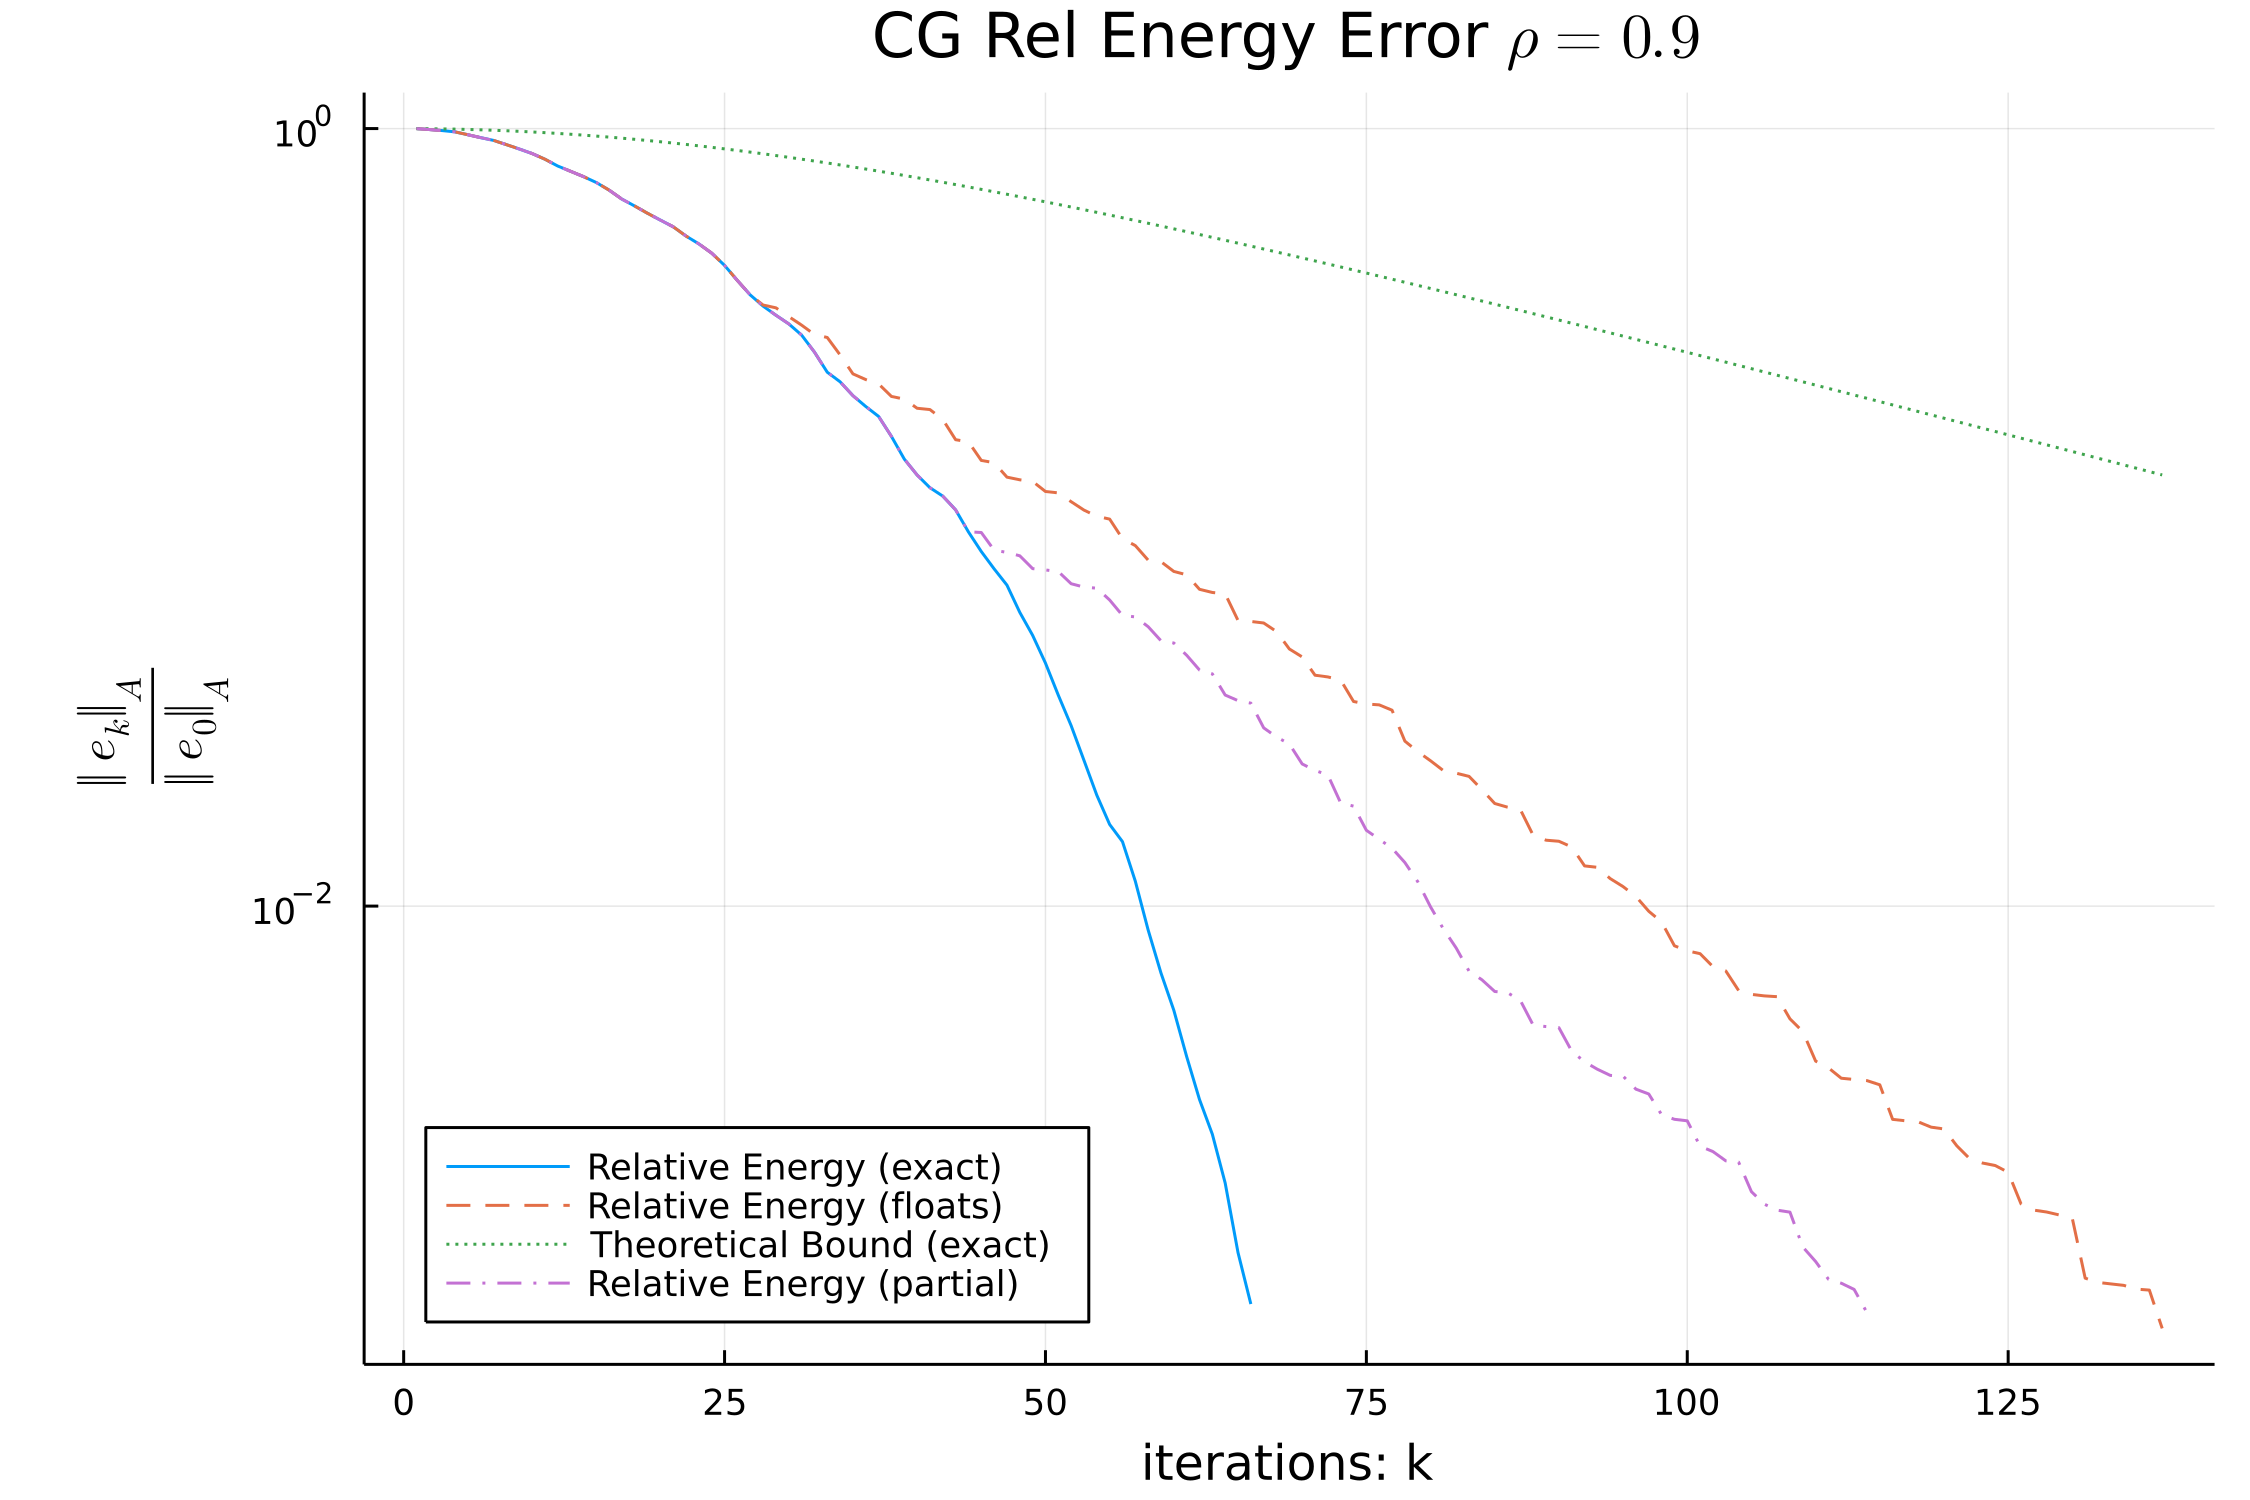
\includegraphics[width=20em]{cg_convergence_0.9.png}
                \caption{$\rho = 0.9$}
        \end{figure}
    \end{frame}
    \begin{frame}{Experiment}
        \begin{figure}
            \centering
            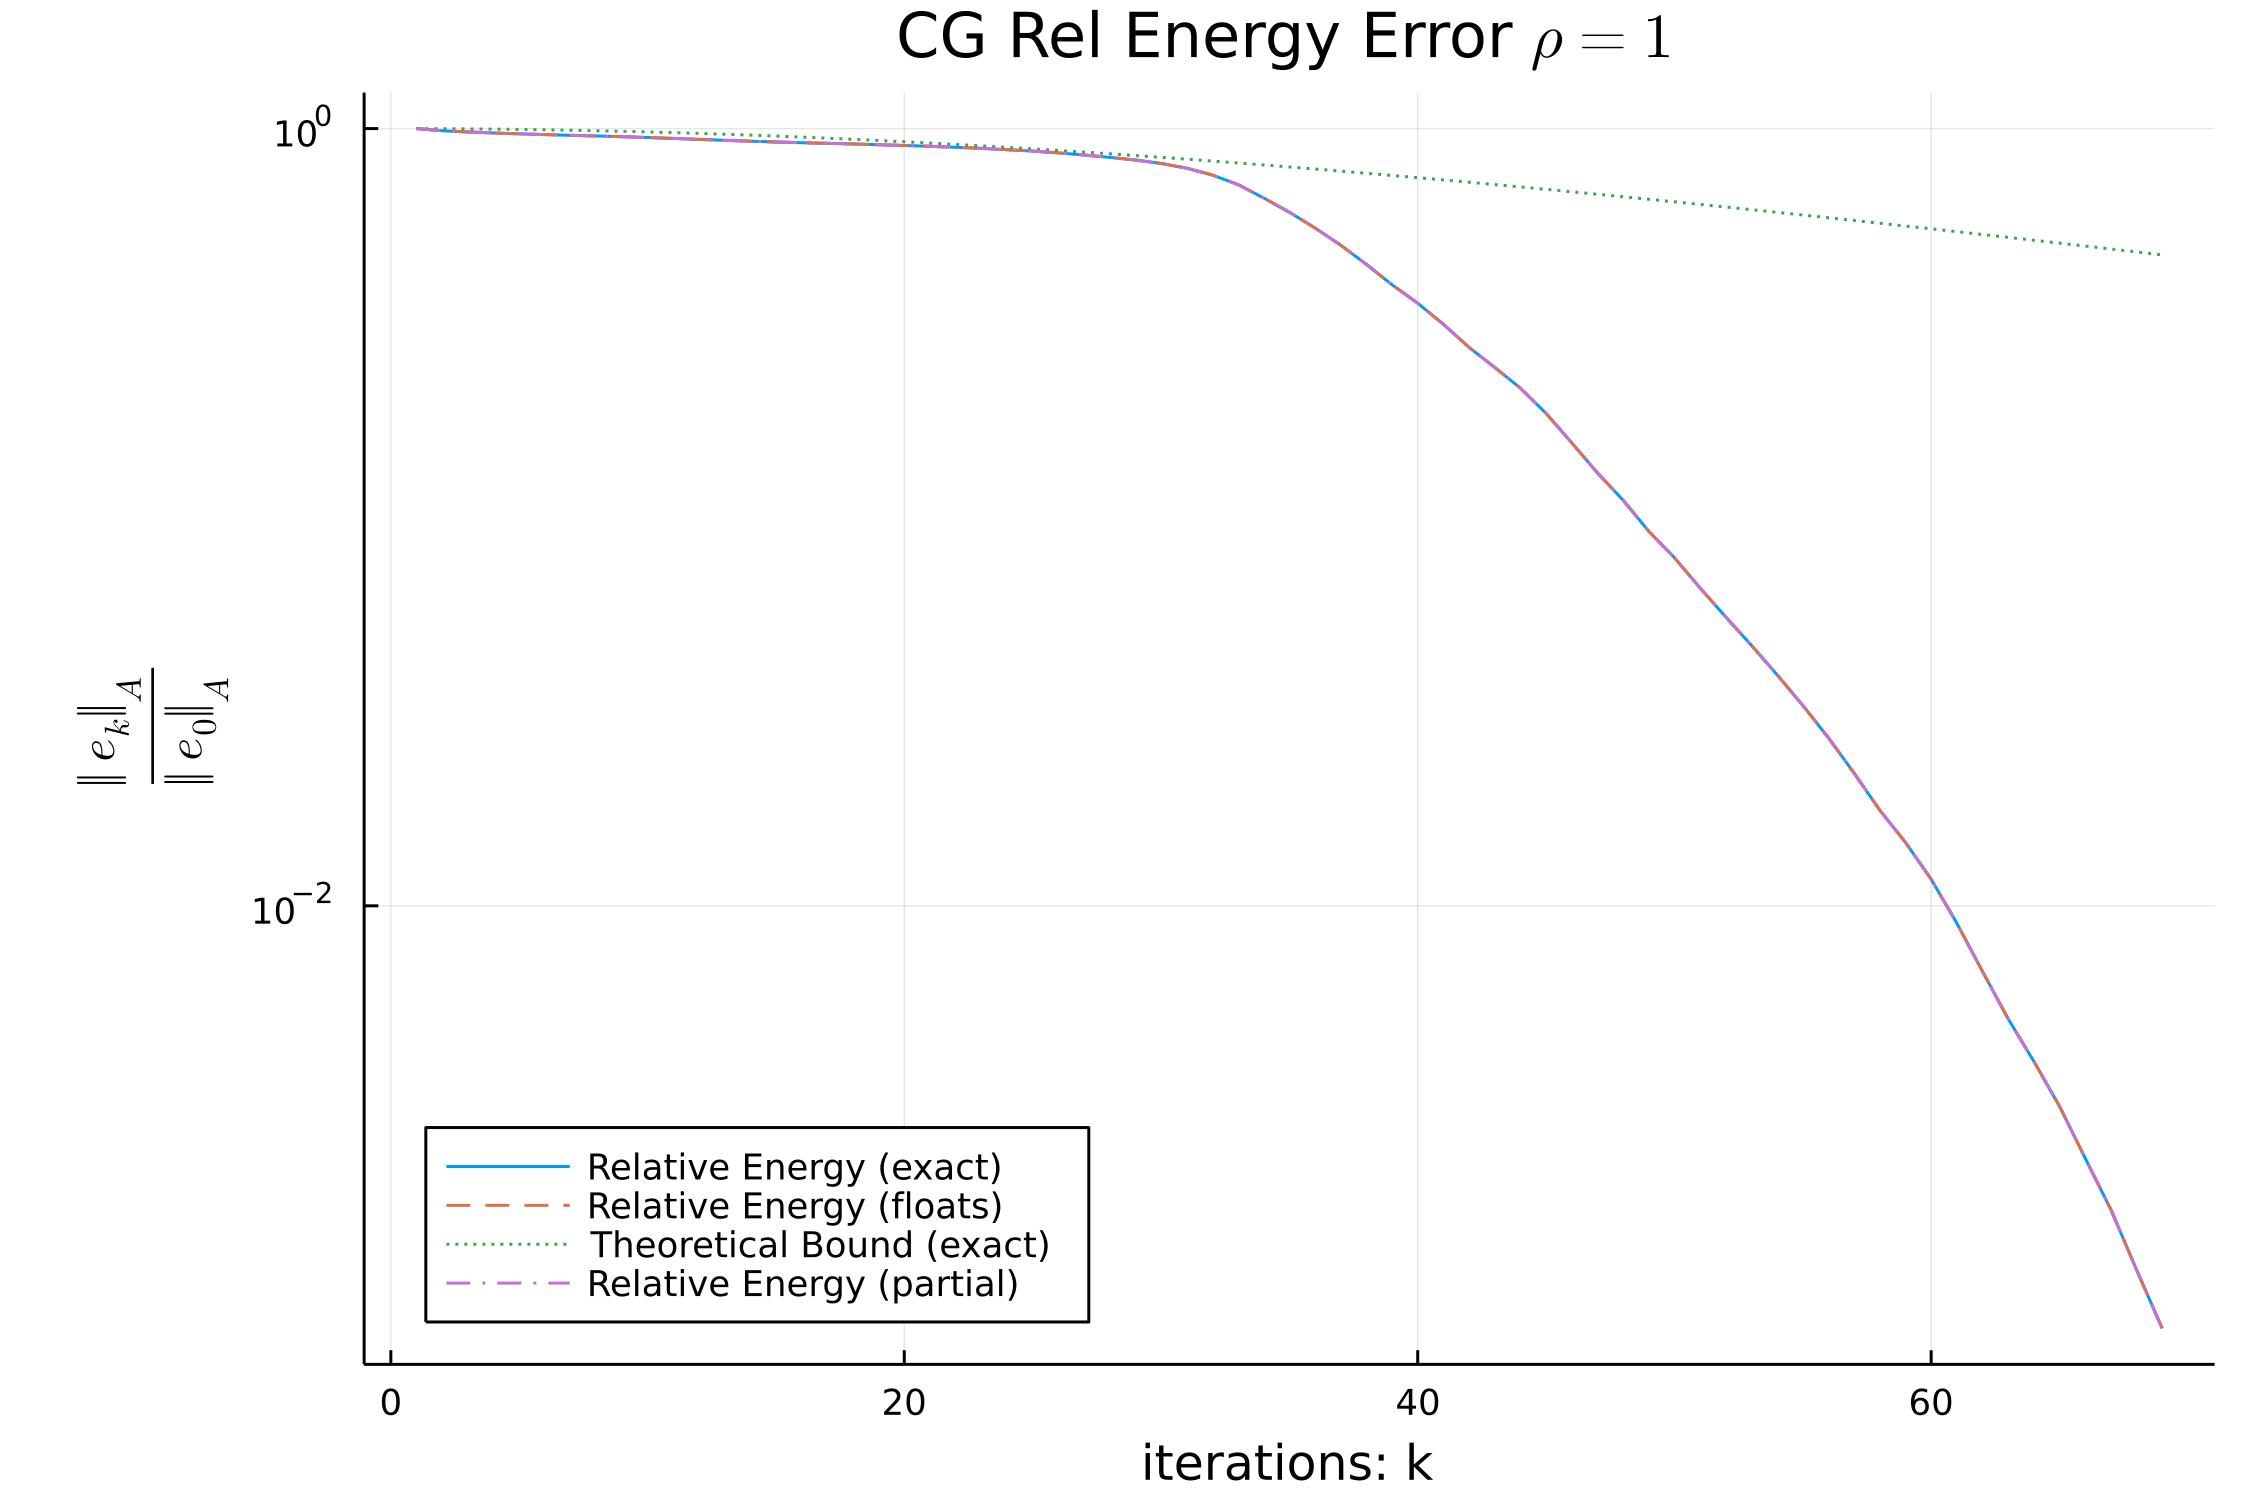
\includegraphics[width=20em]{cg_convergence_1.png}
            \caption{$\rho = 1$}
        \end{figure}
    \end{frame}
    \begin{frame}{Lost of Orthogonality}
        \begin{itemize}
            \item Floats caused CG $p_k, r_k$ to lose conjugacy and orthogonality. 
            \item What is happening to the equivalent Lanczos algorithm when CG's convergence is slowing down?
        \end{itemize}
    \end{frame}
    \begin{frame}{Lanczos and Ghost Eigenvalues}
        We consider the following spectrum of $A$ for an experiment on Lanczos: 
        \begin{align}
            \lambda_i = \left(-1 + \frac{2(i - 1)}{(n - 1)}\right)^3
            \quad 1\le i \le n
        \end{align}\label{eqn:the_ill_conditioned_matrix}
        \begin{itemize}
            \item Symmetric spectrum around origin. 
            \item Tightly clustered eigenvalues around origin, sparse around the boundary. 
            \item $A\in \mathbb R^{64 \times 64}$ and Float64 is used. 
        \end{itemize}
    \end{frame}
    \begin{frame}{Ghost Eigenvalues Plot}
        \begin{figure}[H]
            \centering
            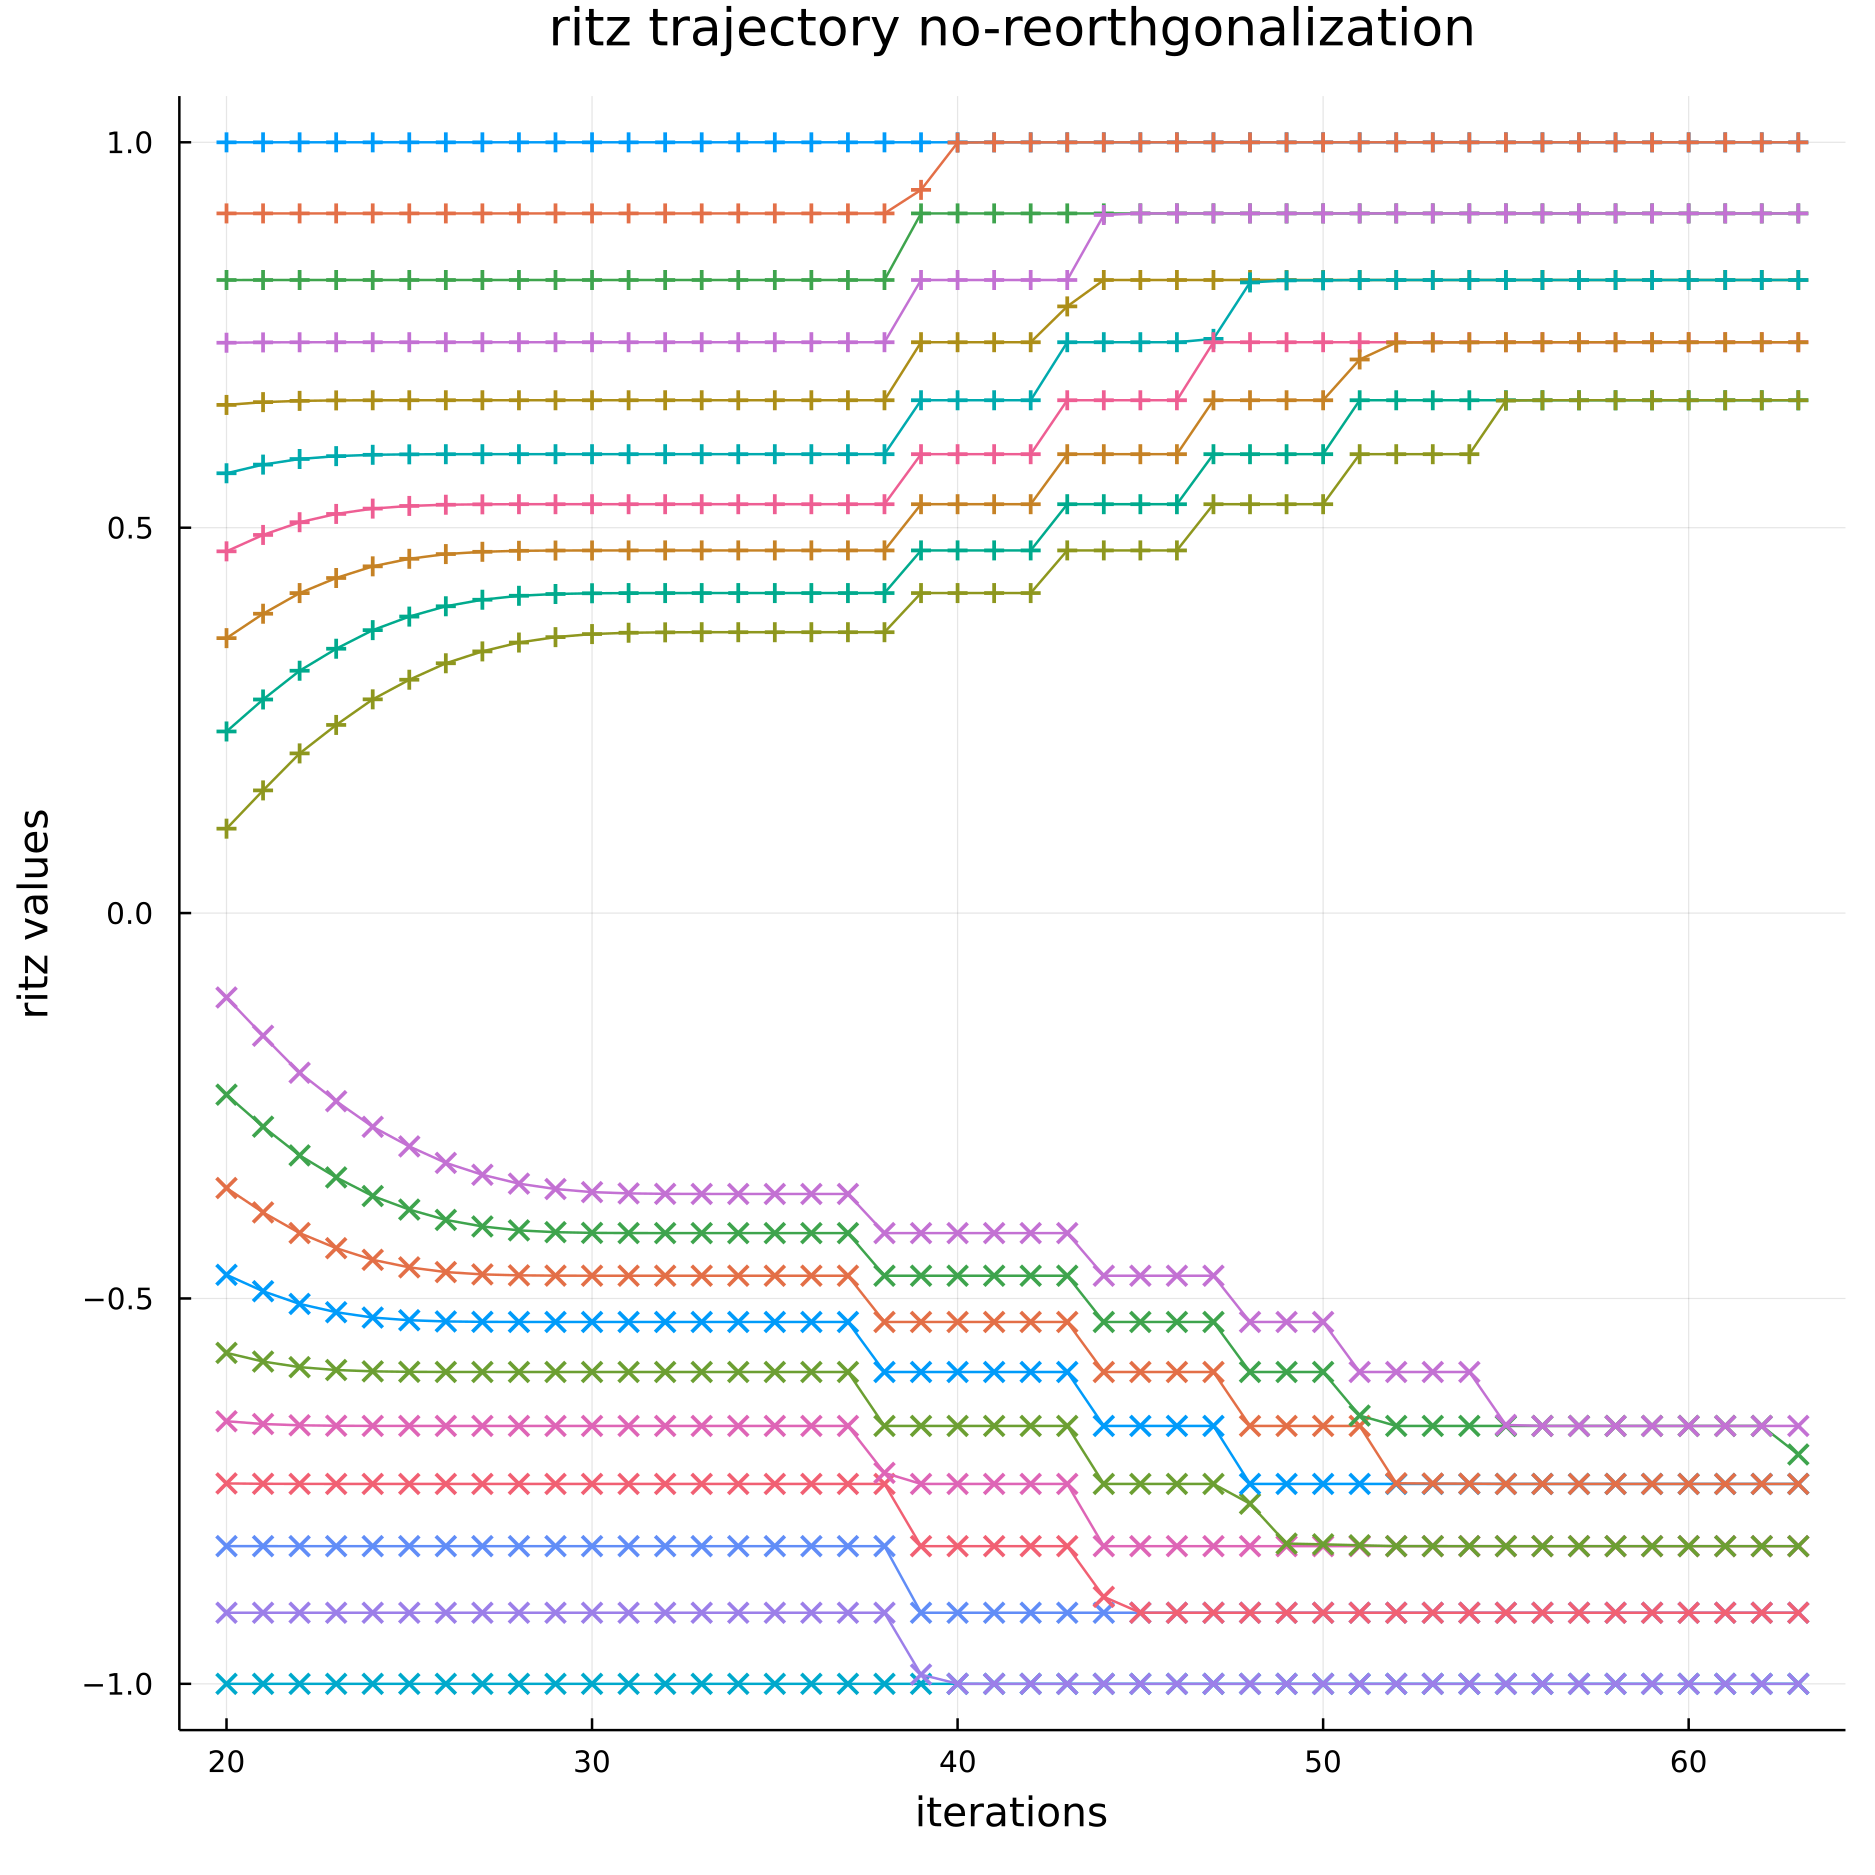
\includegraphics[width=8cm]{ritz_trajectory_plot_floats.png}
        \end{figure}
    \end{frame}
    \begin{frame}{Ghost Eigenvalues Plot}
        \begin{figure}
            \centering
            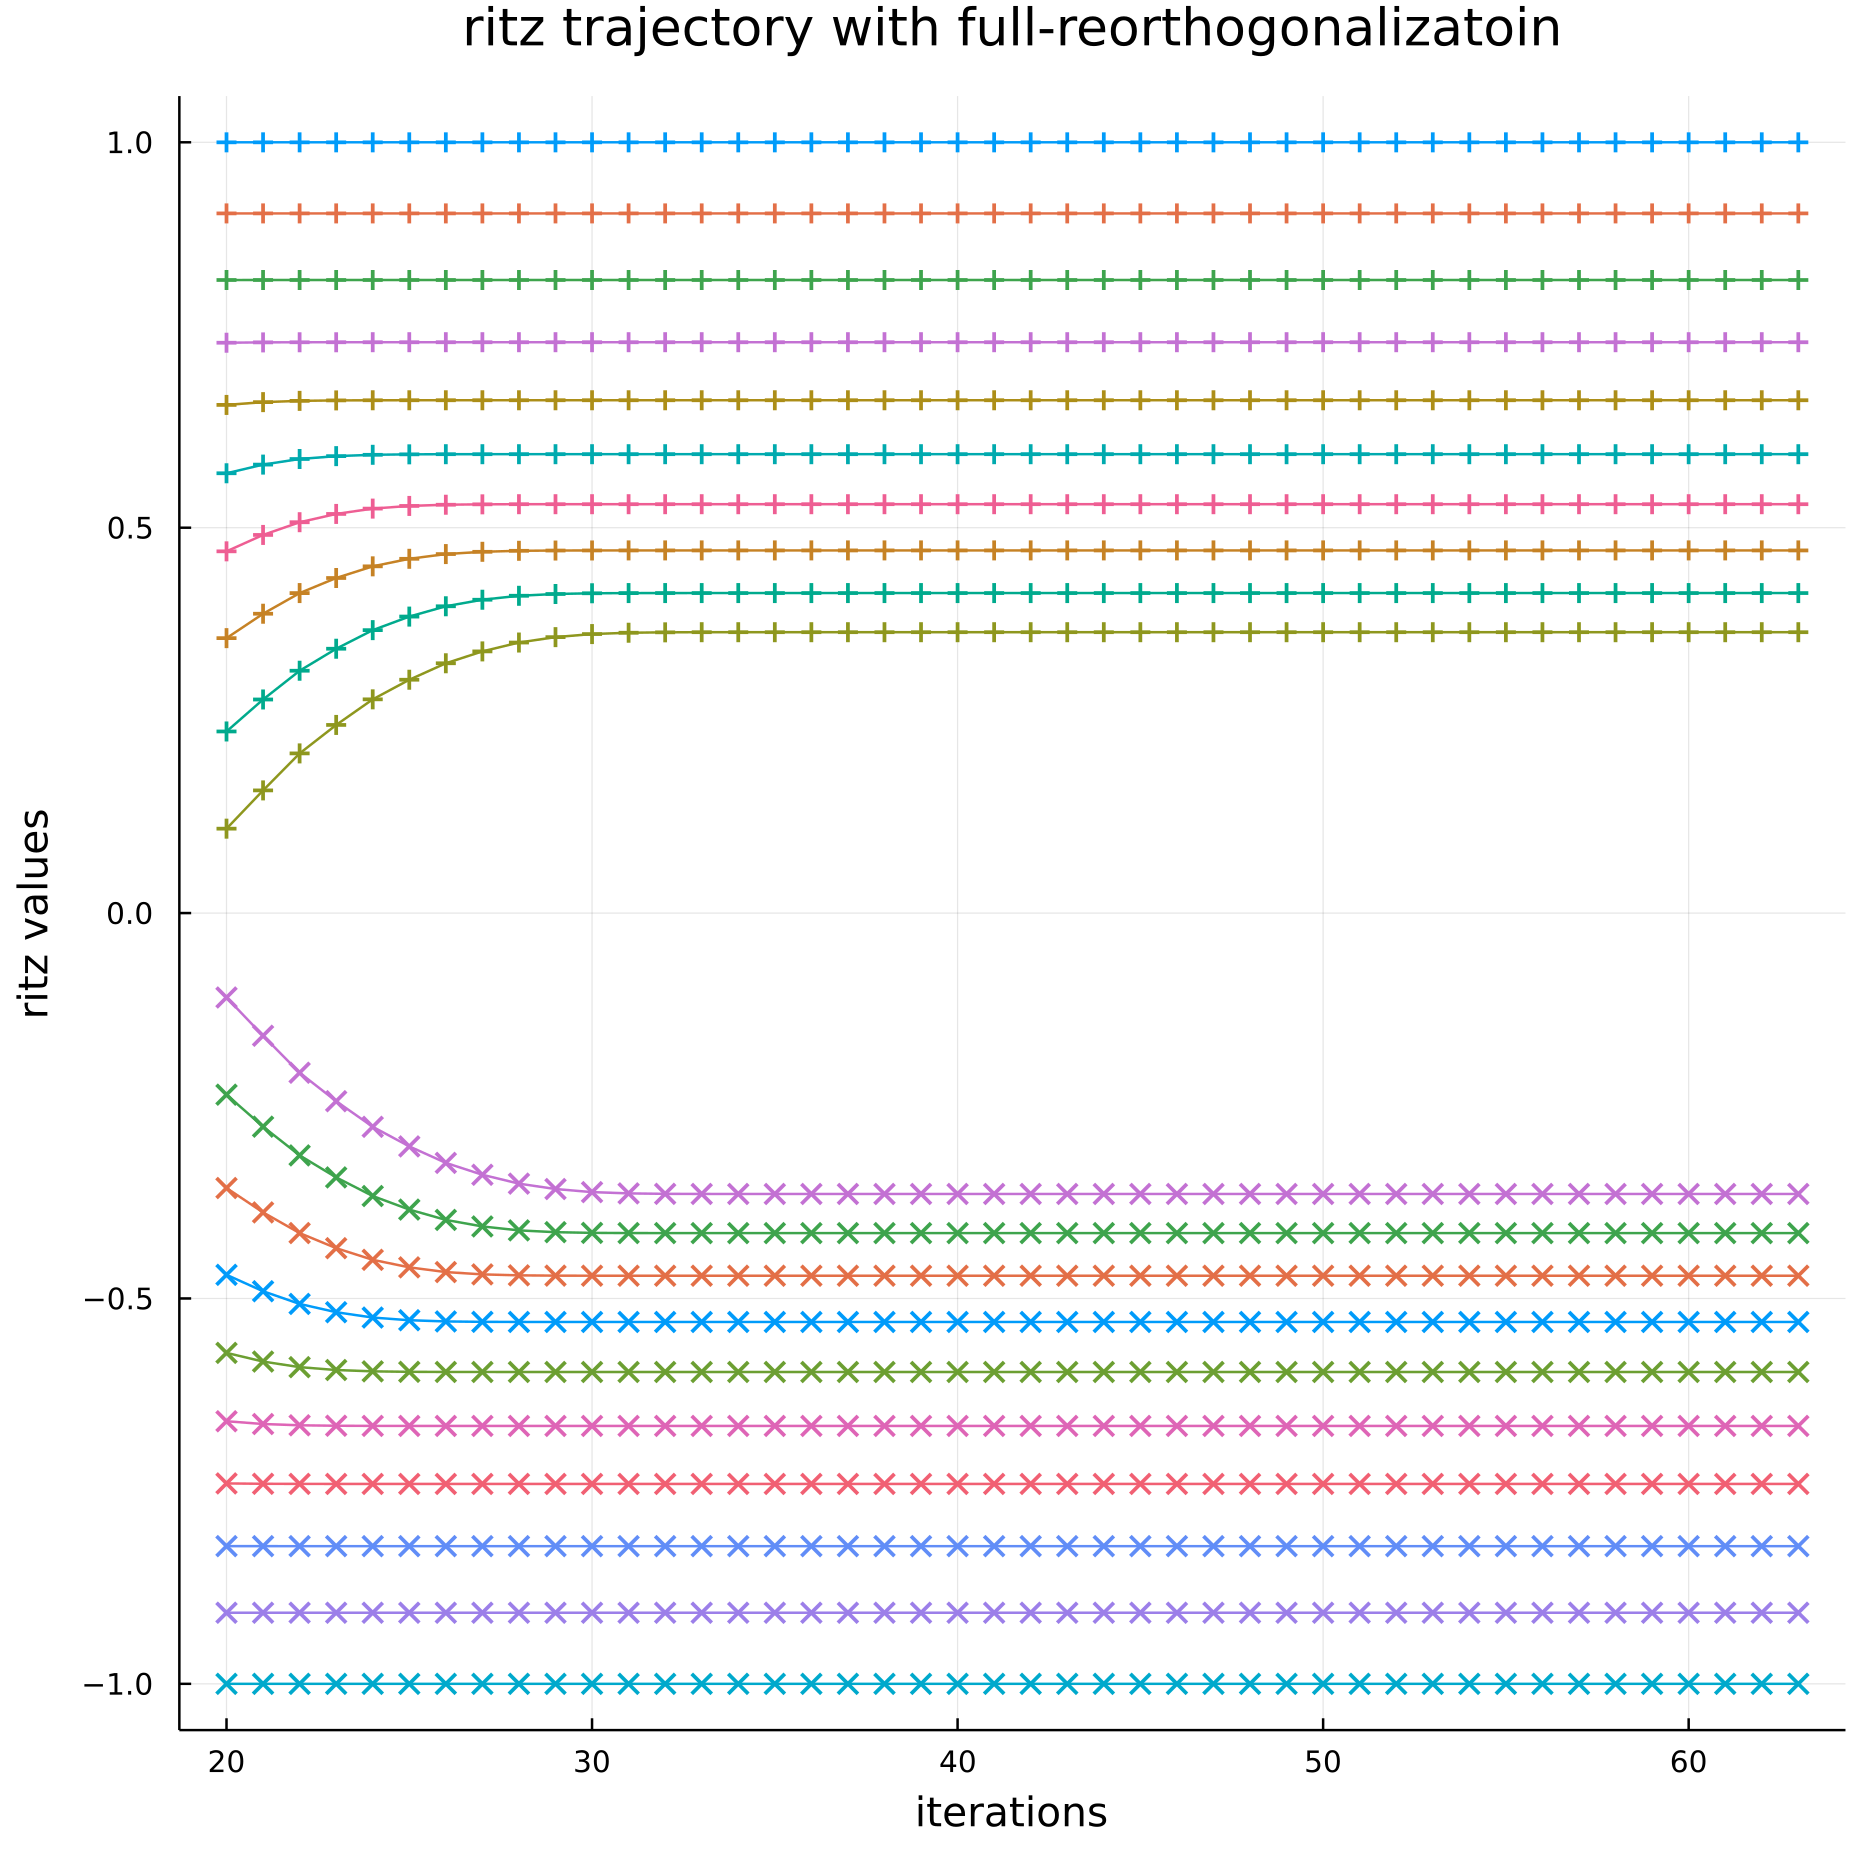
\includegraphics[width=8cm]{ritz_trajectory_plot_exact.png}
        \end{figure}
    \end{frame}
    \begin{frame}{Lost of Orthogonality}
        \begin{figure}[H]
            \centering
            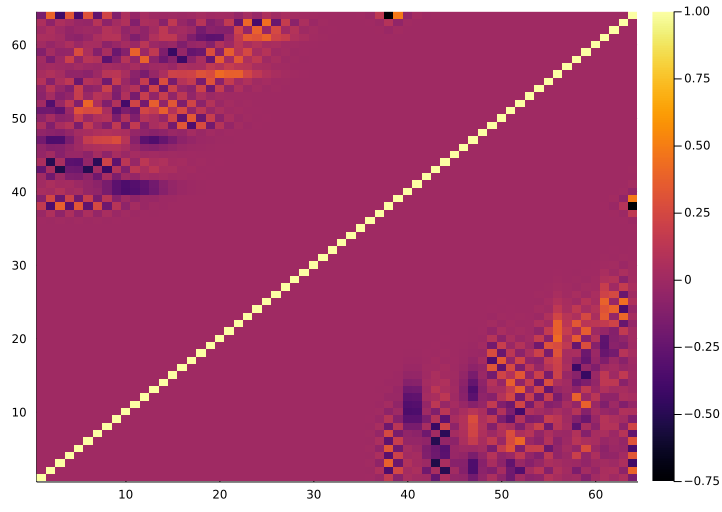
\includegraphics[width=12em]{fig3.png}
            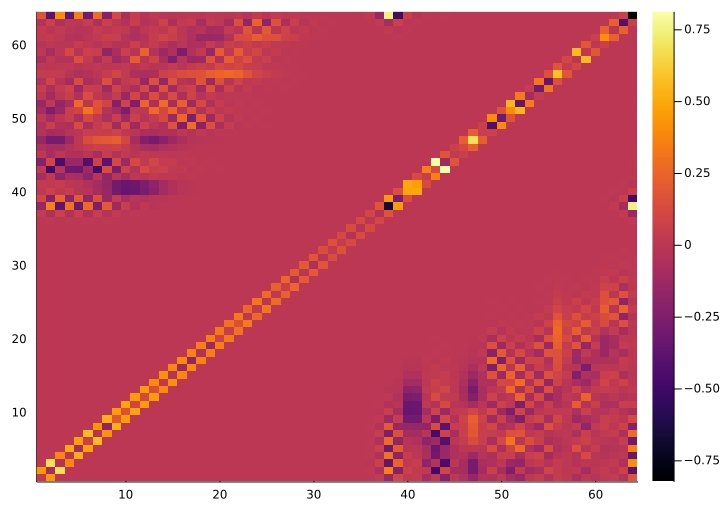
\includegraphics[width=12em]{fig4.png}
             \caption{left: The heatmap of the plot of the absolute values of the matrix $Q^T_kQ_k$. right: The plot of $Q_k^TAQ_k$ from floating-point Lanczos iterations}
        \end{figure}
        \begin{itemize}
            \item Ghost eigenvalues effects doesn't imply lost of orthogonality!
            \item It's possible that the trajectory stays stable and then suddenly shifted away, it's called misconvergence. (Reliable Numerical Computations ch1\cite{book:reliable_computation})
        \end{itemize}
    \end{frame}
\section{Diving Deeeeper}
    \begin{frame}{Good news}
        C.C Paige 1980\cite{paper:paige1980} Showed that: 
        \begin{align}
            AQ_k = Q_{k + 1} 
            \begin{bmatrix}
                    T_k
                    \\
                    \beta_k \xi_k^T
            \end{bmatrix} + F_k
        \end{align}
        Still holds good under floating point arithematic, and $F_k$ is a matrix having $\mathcal O(\Vert A \Vert)$ condition numbers. 
    \end{frame}
    \begin{frame}{CG Float Bound}
        Big idea is: 
        \par
        if we were to perform an CG on the $T_{k + 1}$ produced by the finite precision algorithm with the initial Lanczos vector $q_1$ being $\xi_1^{(n)}$, then its residual $\overline{r}_{k}$ of equivalent CG would be exact and it's given as $-\beta_kT_{k}^{-1}\xi_kq_{k + 1}$, but with $q_{k + 1} = \xi_{k + 1}^{(n)}$, the $k + 1$ th standard basis vector in $\mathbb R^{n}$, and $T_k = (T_{k + 1})_{1:k, 1:k}$. 
        \begin{itemize}
            \item We use exact convergence to bound that quantity. 
            \item $-\beta_kT_{k}^{-1}\xi_kq_{k + 1}$ shows up as the residual of CG using Lanczos under floating point arithematic.
            \item It's also how we show that: "Ghost eigenvalue effects doesn't neccessarily imply lost of orthogonality". 
            \item Paige used this idea (and his 1980 paper on Lanczos iterations) to give a convergence rate for CG under floating point arithematic as well. 
        \end{itemize}
    \end{frame}
    \begin{frame}{Losting orthogonality On Ritzvectors}
        Firstly, we need to know what we expect when eigenvalues of $T_k$ is close to an eigenvalue of $A$. 
        \begin{align}
            AQ_k &= Q_k T_k + q_{k + 1}\beta_k\xi_k^T
            \\
            AQ_ks_i^{(k)} &= \theta_j^{(k)} Q_k s_i^{(k)} + q_{k + 1}\beta_k \xi_k^Tv
            \\
            AQ_ks_i^{(k)} &= \theta_j^{(k)} Q_k s_i^{(k)} + \beta_kq_{k + 1}(s_i^{(k)})_k
            \\
            AQ_ks_i^{(k)} - \theta_j^{(k)} Q_k s_i^{(k)} &=   \beta_kq_{k + 1}(s_i^{(k)})_k
        \end{align}
        Note, $q_k^TQ_ks_i^{(k)} = (s_i^{(k)})_k$ under exact arithematic. $Q_ks_i^{(k)}$ Approximates eigenvector of $A$ (it's exact under the subspace spanned by $Q_k$), it's called the Ritzvectors. How does this work in floating point arithematic? 
    \end{frame}
    \begin{frame}{Losing Orthogoality on Ritzvectors}
        \begin{figure}[H]
            \centering
            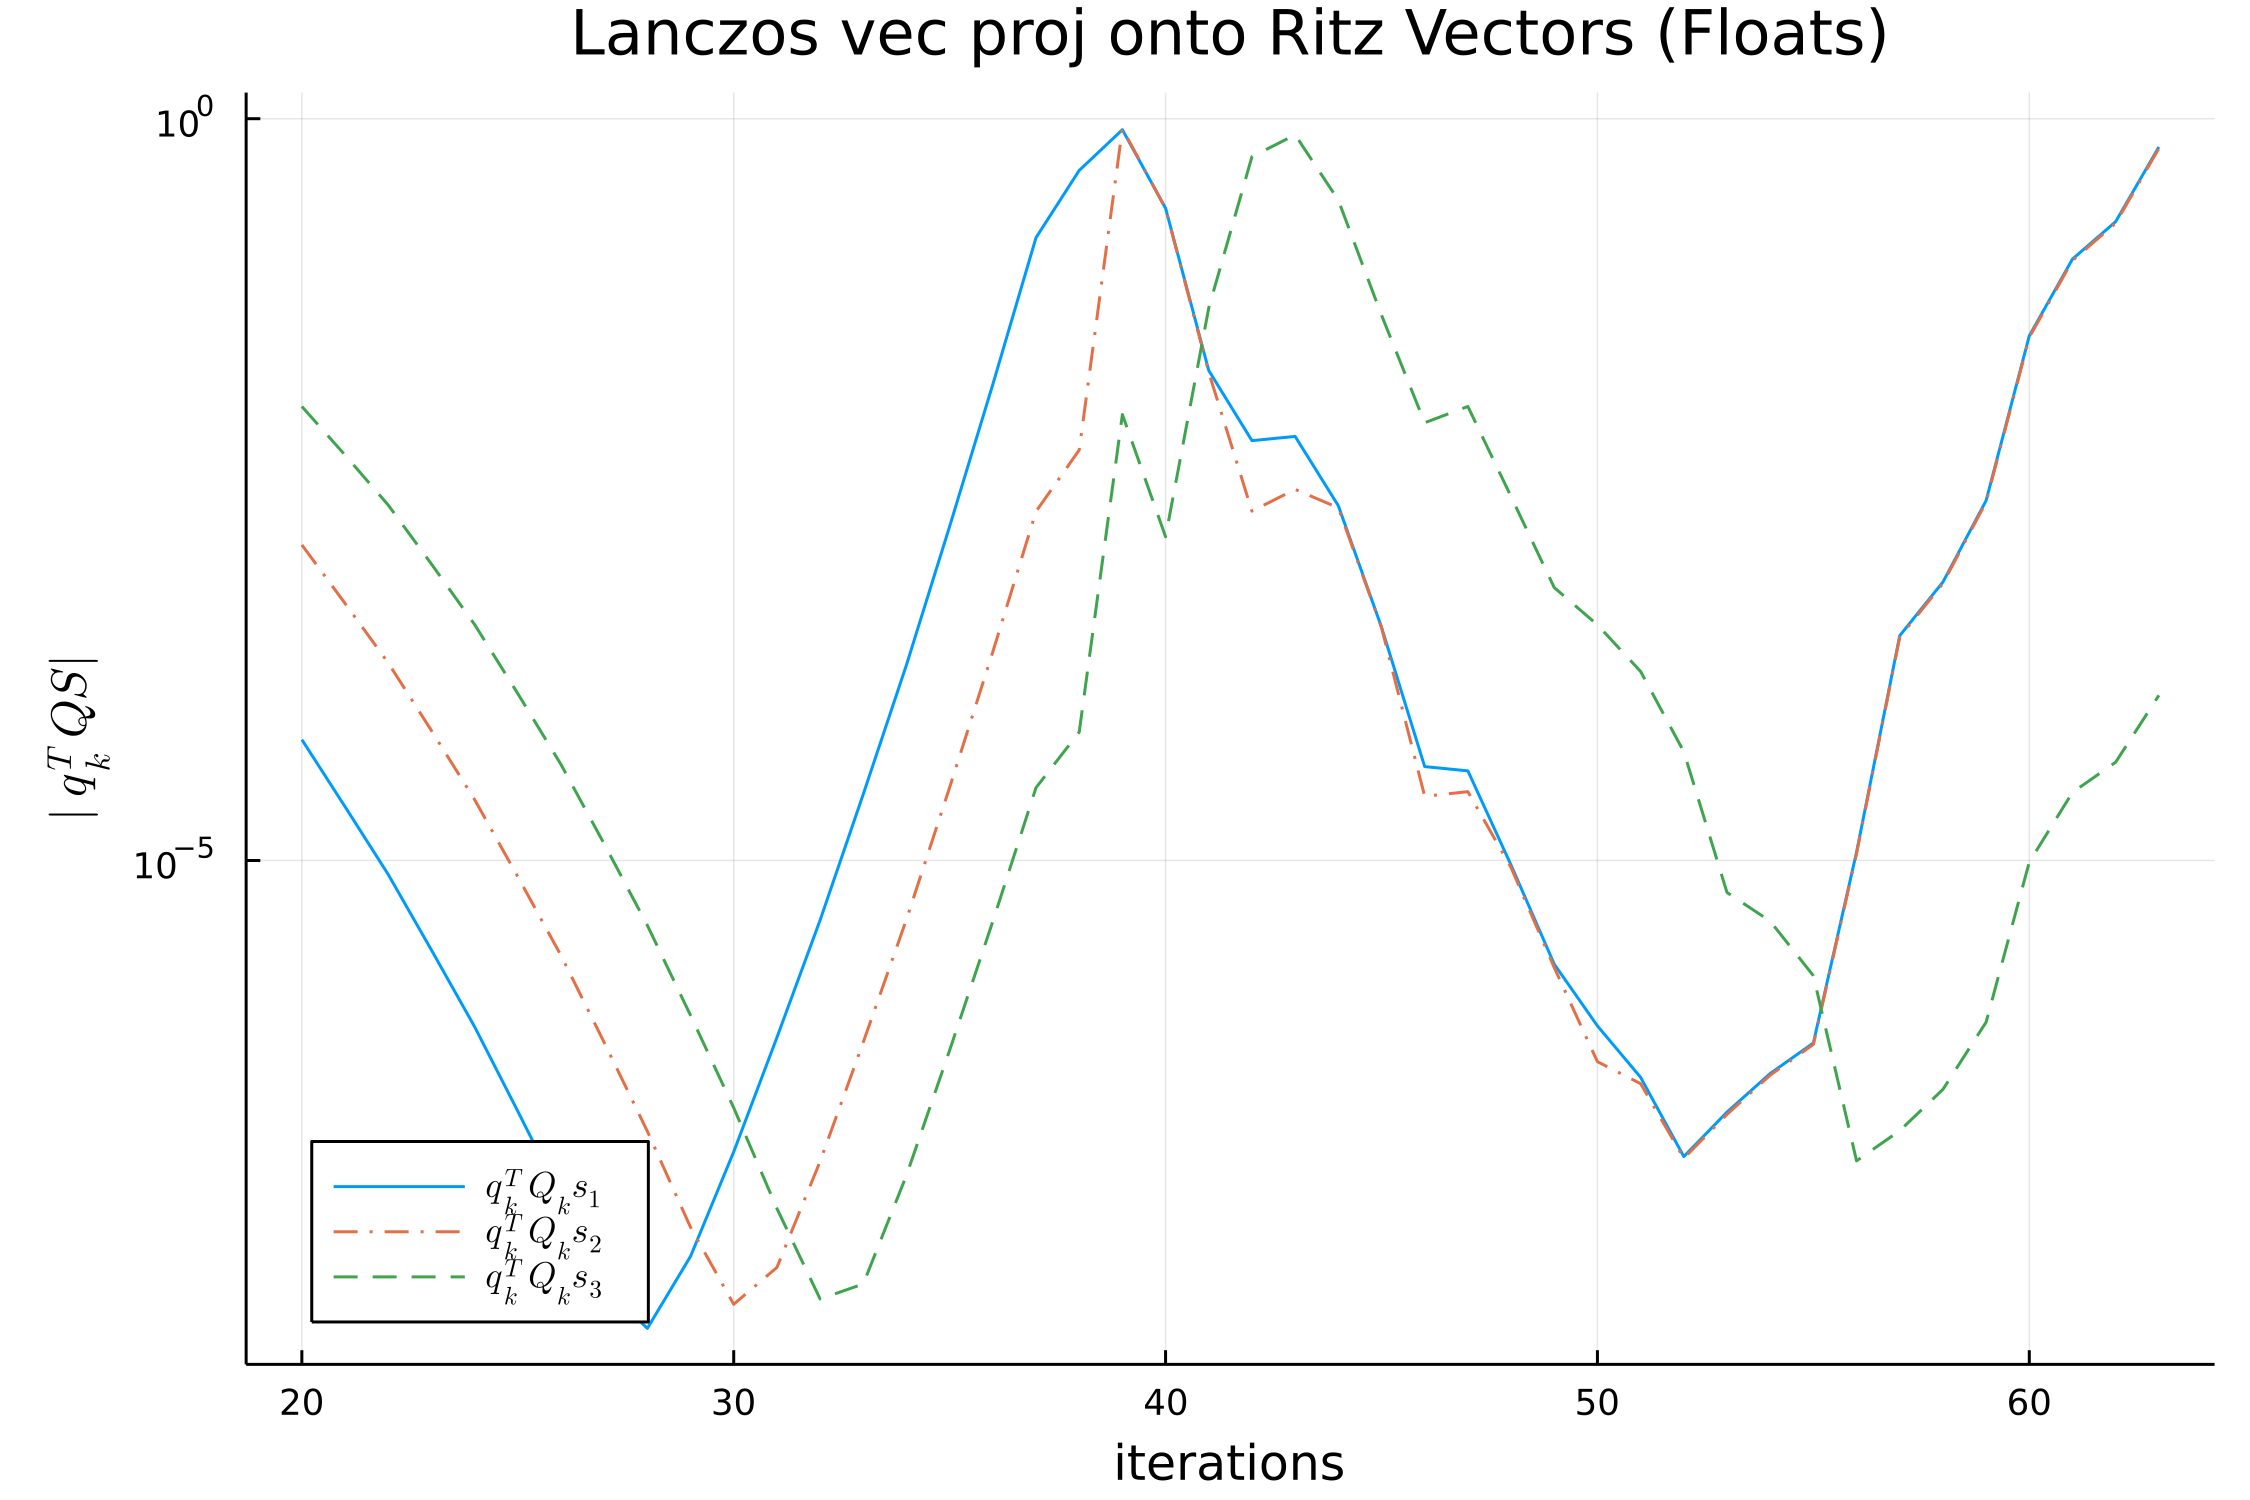
\includegraphics[width=20em]{lanczos_proj_on_ritz_float.png}
            \caption{Projection of floating-point Lanczos vector $q_k$ onto 3 of the largest Ritz vectors: $Q_ks_i^{(k)}$, for $i = k, k - 1, k - 2$
            }
        \end{figure}
    \end{frame}
    \begin{frame}{Losing Orthogoality on Ritzvectors}
        \begin{figure}[H]
            \centering
            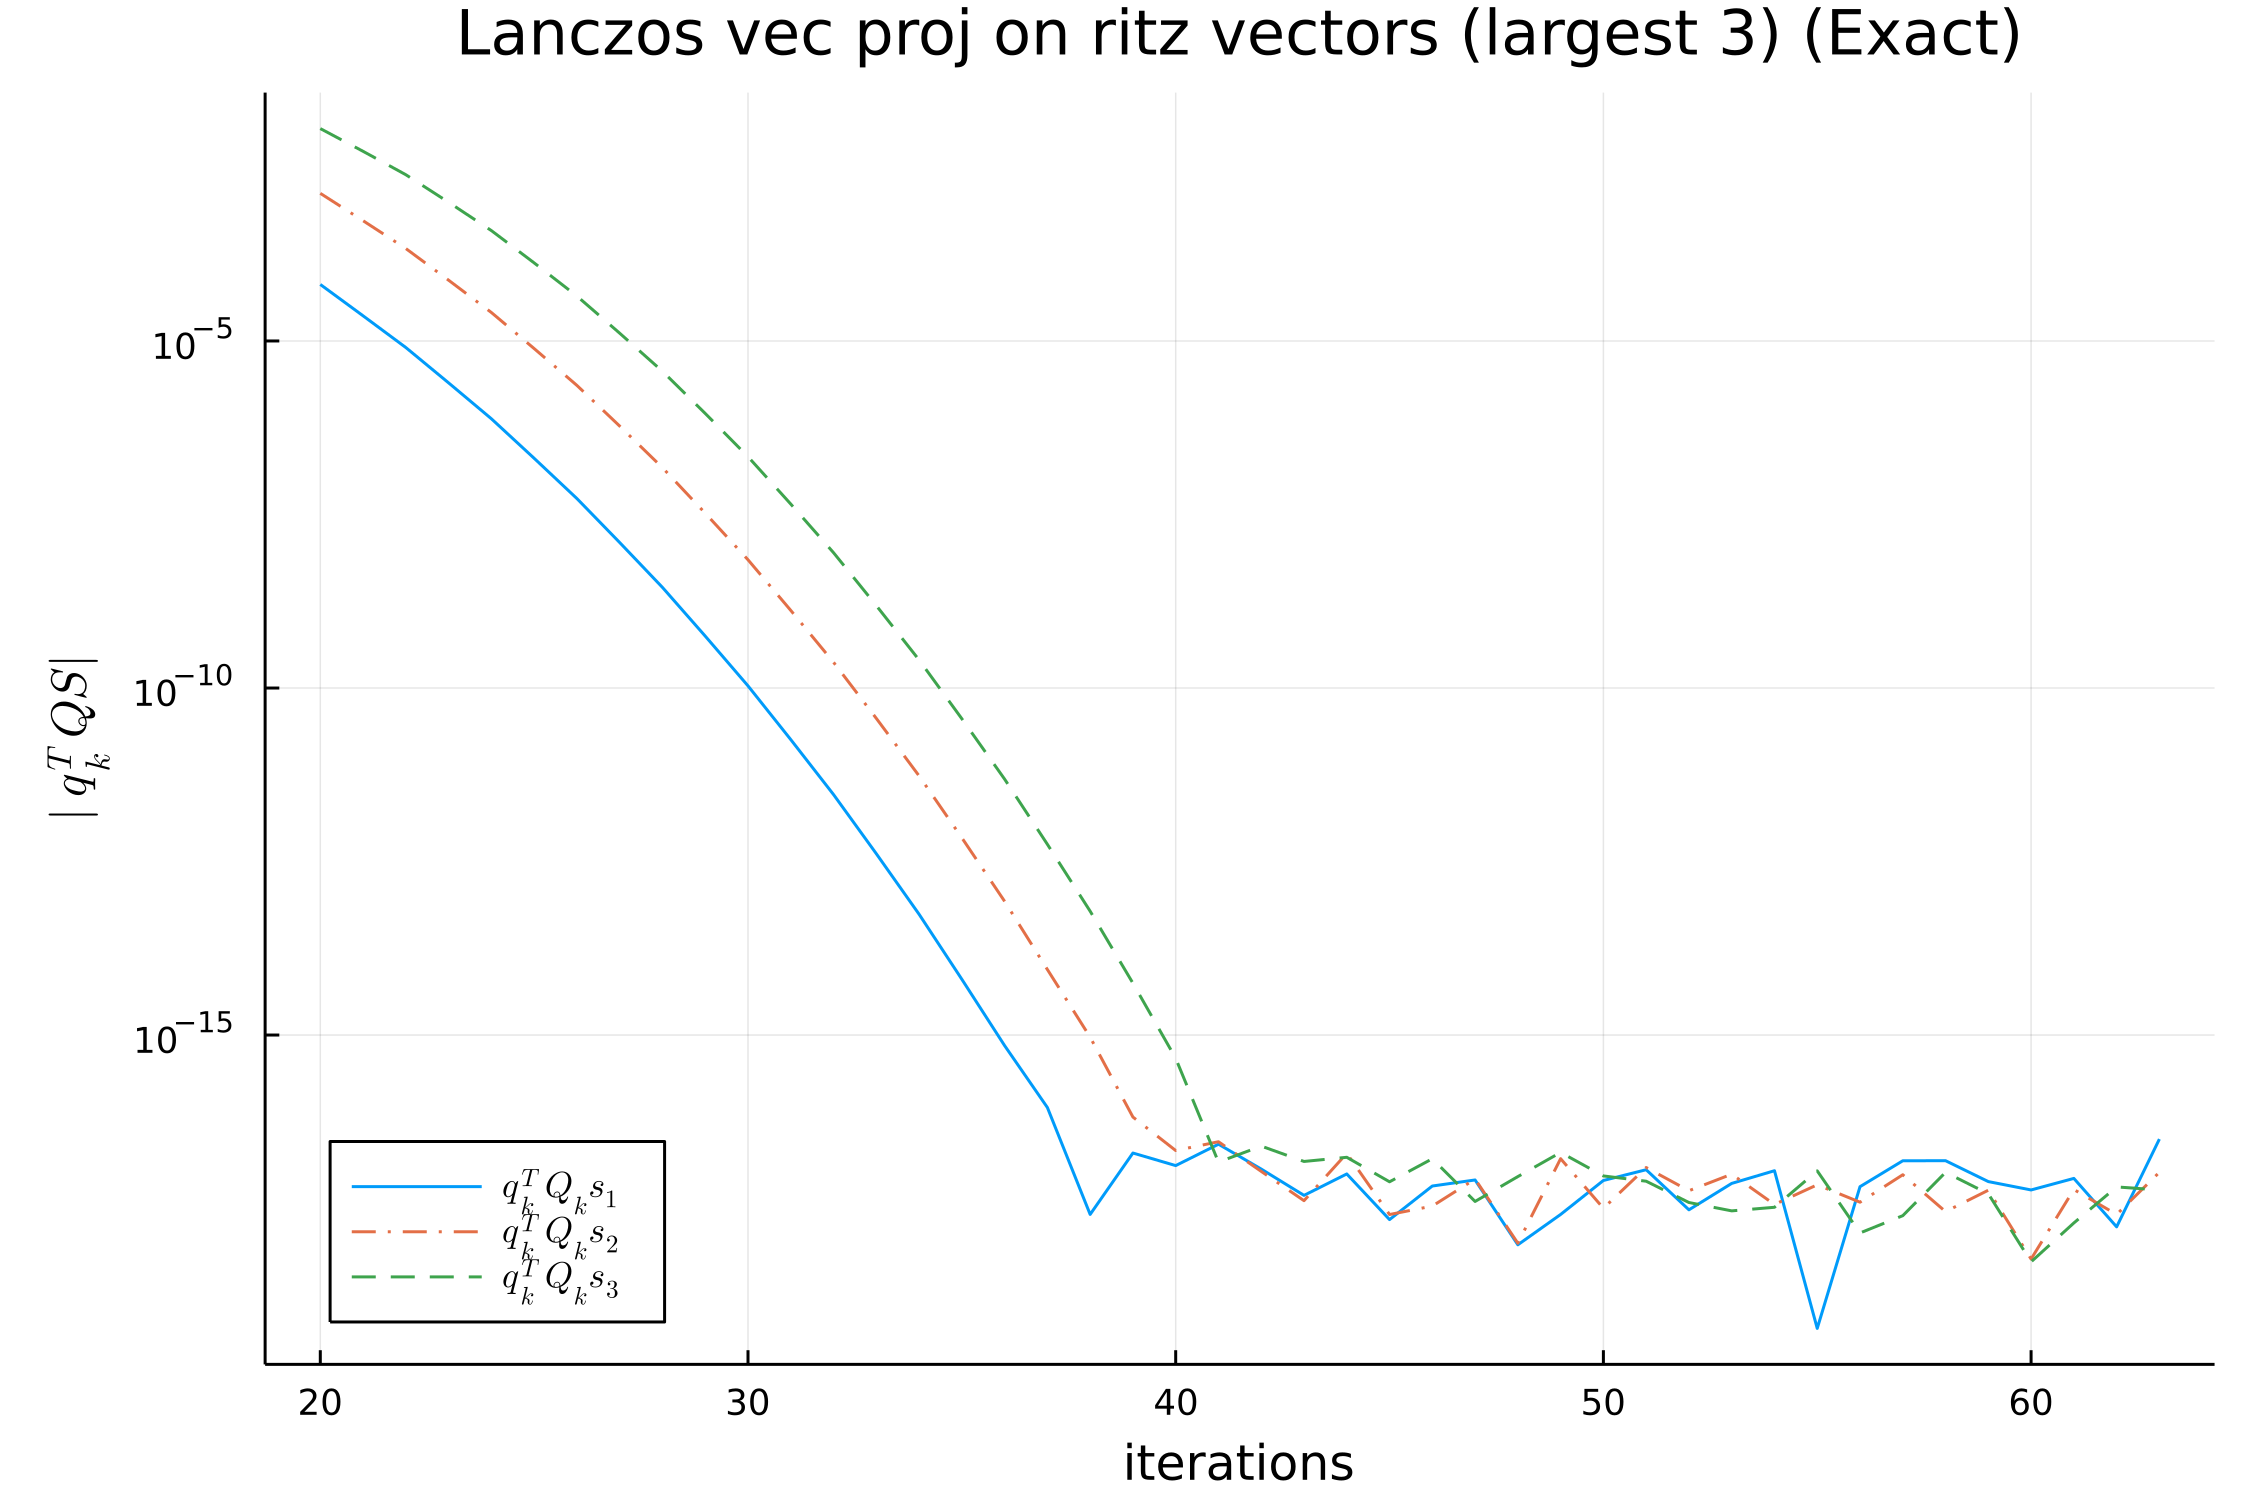
\includegraphics[width=20em]{lanczos_proj_on_ritz_exact.png}
            \caption{projection of the exact Lanczos vector $q_k$ onto 3 of the largest Ritz vectors: $Q_ks_i^{(k)}$, for $i = k, k - 1, k - 2$}
        \end{figure}
    \end{frame}
    \begin{frame}{Losing Orthogonality on Ritzvectors}
        \begin{figure}[H]
            \centering 
            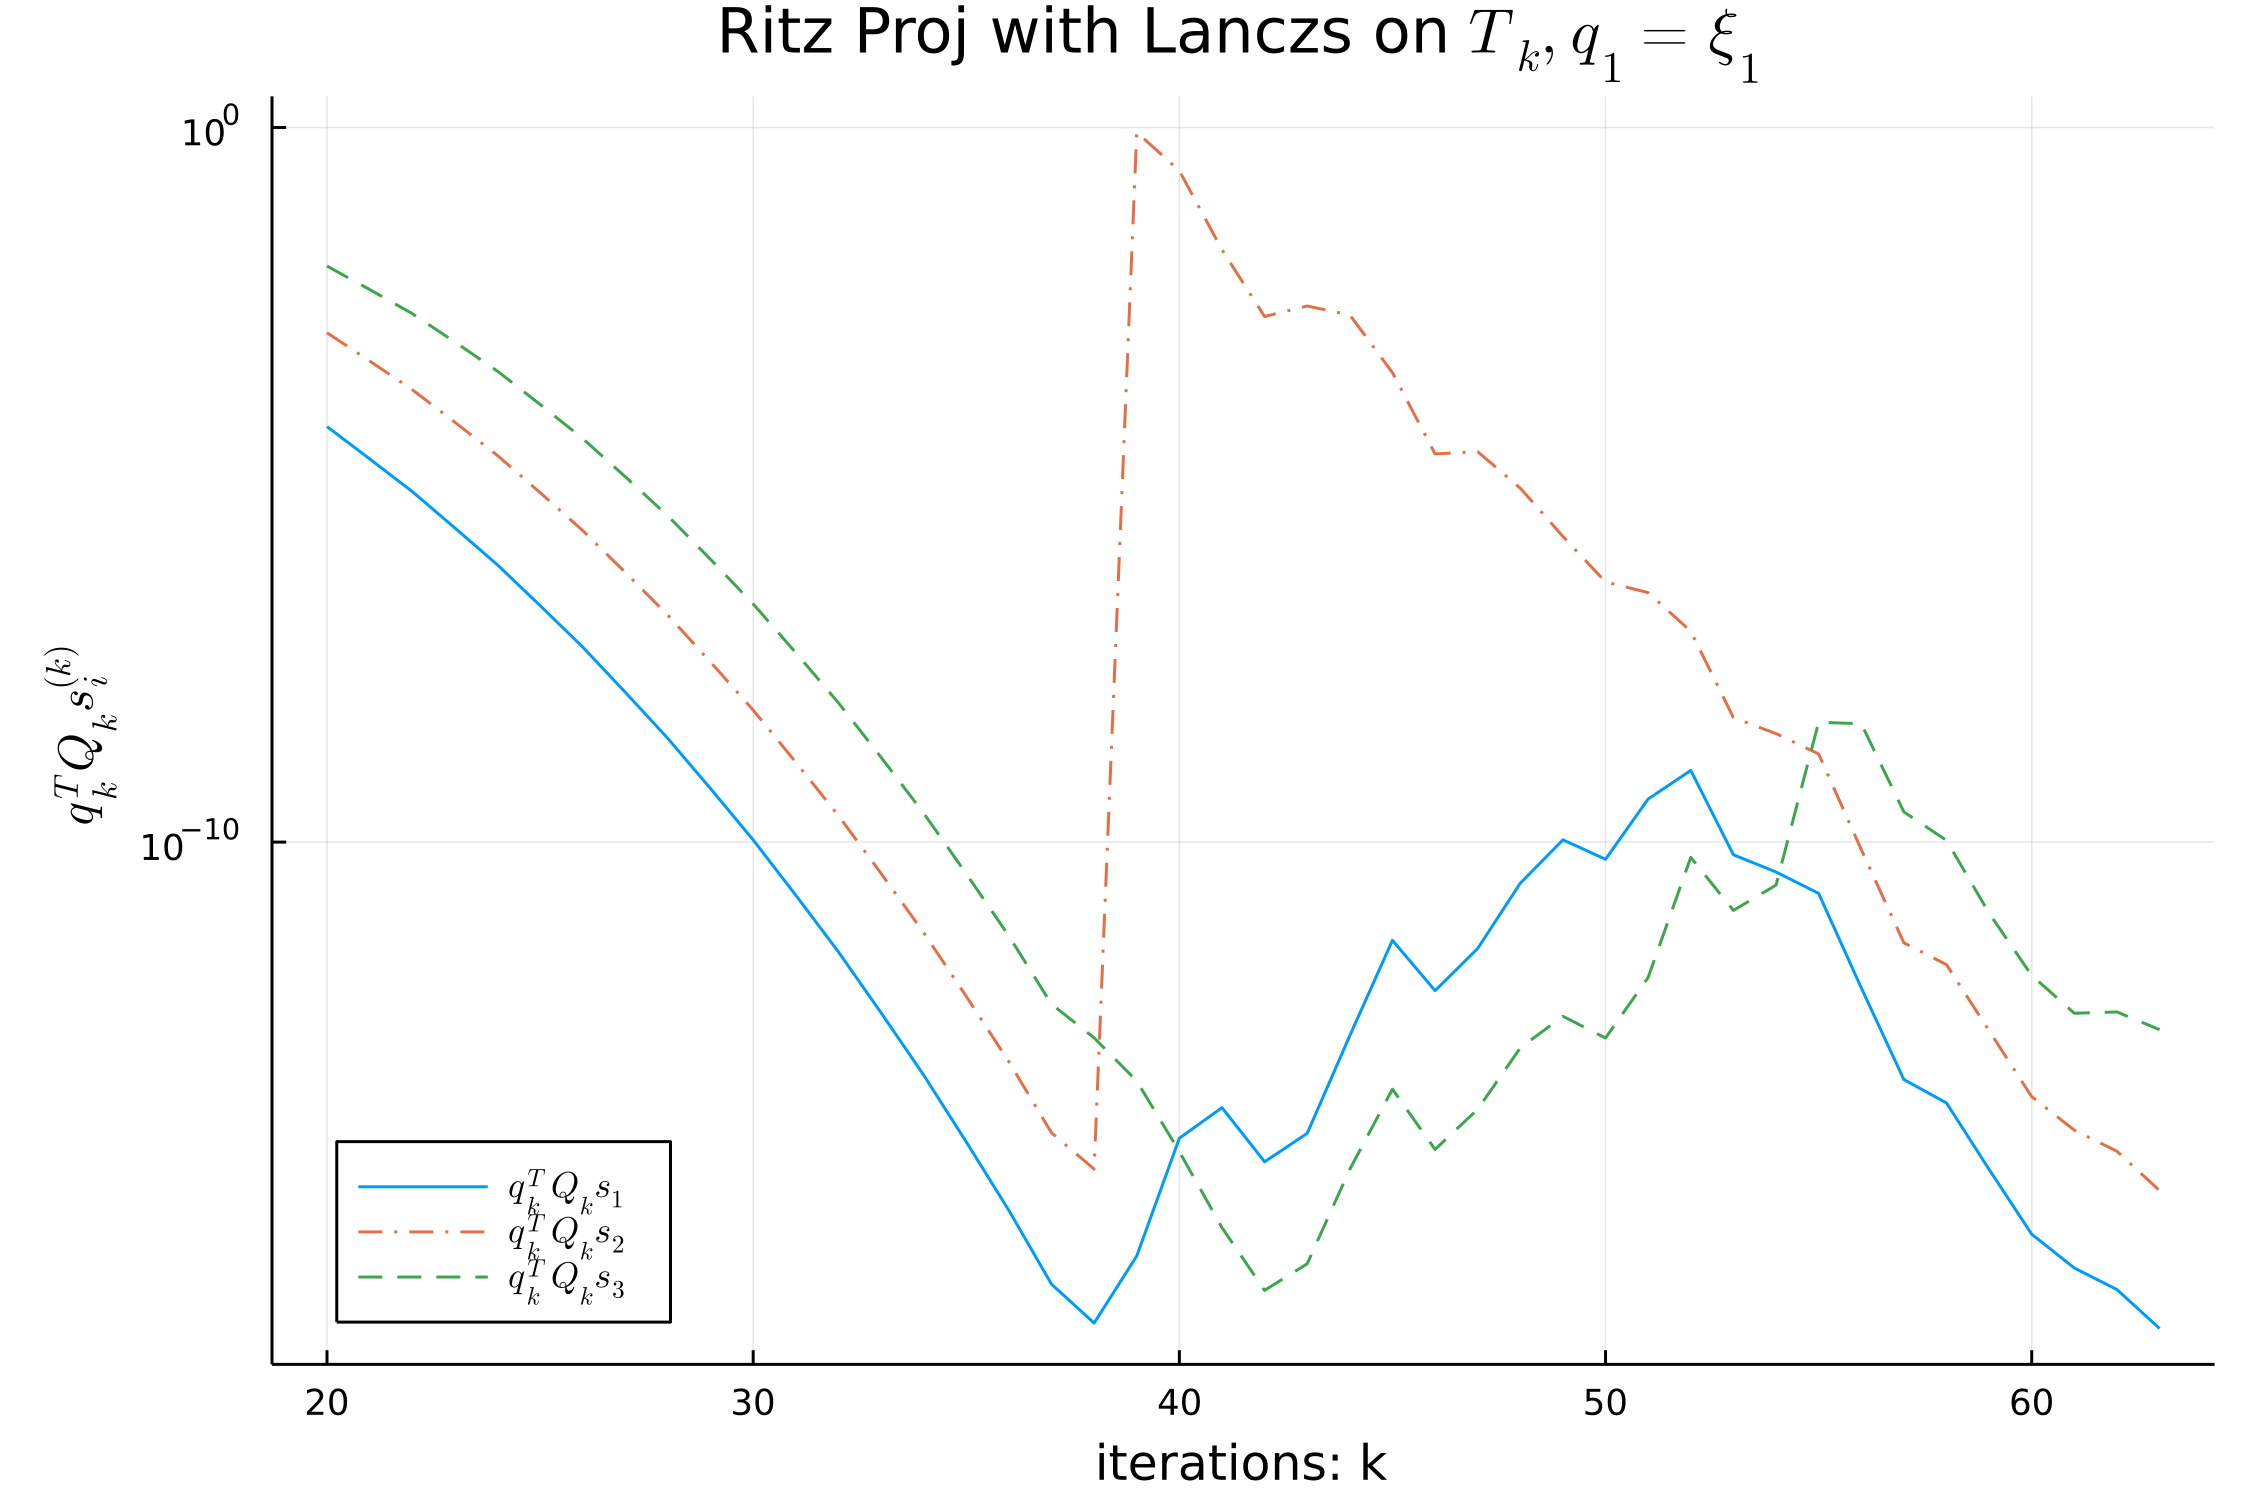
\includegraphics[width=20em]{ritz_proj_tridiagonal.png}
            \caption{The projection of most recent Lanczos vector $q_k$ onto the first 3 Ritzvectors: $Q_ks_i^{(k)}$ for $1\le i \le 3$, it's performed on a Tridiagonal matrix $T_k$ generated by finite precision lanczos with $q_1 = \xi_1$. }
        \end{figure}
    \end{frame}
    \begin{frame}{Losing Orthogonality on Ritzvectors: Final Remark}
        \begin{itemize}
            \item The Lanczos recurrences are not affected by much due to floating point error, which it's exploited for matrix function approximations. 
            \item The $Q_k$ generated are not orthogonal any more and it creates ghost eigenvalues. But we know it's losing orthogonality against ritzvectors. 
            \item Ritzvalues can converge several times. 
        \end{itemize}
    \end{frame}
    \begin{frame}{Tiny Intervals}
        Take advantage of the clustering of the ghost eigenvalues and think of them as the eigenvalues of a potentially a larger matrix, denoted as $\tilde{A}$ whose eigenvalues are clustered around the eigenvalues of $A$ within a tiny interval. Due to the effect of round of errors, the floating-point Lanczos iterations can't see the spectrum of $A$ clearly and instead, it sees $\tilde{A}$ whose eigenvalues are smeared out version of $A$, and there are many of them clustered around. More specifically, assuming $A$ has eigenvalues: $\lambda_1, \cdots, \lambda_n$, the eigenvalues of $\tilde{A}$ lies in: 
        \begin{align}
            \bigcup_{n = 1}^n[\lambda_i - \delta, \lambda_i + \delta]
        \end{align}
    \end{frame}
    
    \begin{frame}{Tiny Intervals}
        Experiments of tiny intervals were carried out by Greenbaum, Strakos\cite{paper:greenbaum_tiny_interval_experiments}. We replicate the experiment here for CG. 
        \begin{itemize}
            \item $\delta = \text{2e-5}\Vert A\Vert \epsilon$ 
            \item 100 equally spaced eigenvalues on the spectrum for the matrix $\tilde A$
            \item $A\in \mathbb R^{64\times 64}$
        \end{itemize}
    \end{frame}
% \section{Problem Setup}
%     \begin{frame}{MDP from Susceptible-Exposed-Infectious-Recovered (SEIR) model}
%         \begin{itemize}
%             \item \textbf{States}: $\mathcal{S} = \{(p_S, p_E, p_I) \in \mathbb{R}_+^3 \hspace{1mm} | \hspace{1mm}  p_S + p_E + p_I \le 1 \}$, where:
%             \begin{itemize}
%                 \item $p_S,p_E,p_I$ are the proportion of susceptible, exposed, and infectious individuals, respectively
%             \end{itemize}
%             \item \textbf{Actions:} $\mathcal{A} = \{(y_V, y_R) \in \mathbb{N}^2 | y_V \le L, y_R \le M\}$
%             \begin{itemize}
%                 \item $y_V(t) = i$ amount of vaccines distributed vaccines to susceptibles at stage $t$. 
%                 \item $y_R$ is the scale of transmission-reducing interventions
%             \end{itemize}
%         \end{itemize}
%     \end{frame}

\end{document}